\documentclass[11pt,twocolumn,a4paper]{article}

\usepackage[utf8]{inputenc}
\usepackage[T1]{fontenc}
\usepackage{lmodern}
\usepackage[a4paper,margin=2.1cm,columnsep=0.55cm]{geometry}
\usepackage{amsmath,amssymb,amsthm,mathtools}
\usepackage{bm}
\usepackage{mathrsfs}
\usepackage{booktabs}
\usepackage{array}
\usepackage{enumitem}
\usepackage{microtype}
\usepackage{xcolor}
\usepackage{graphicx}
\usepackage{algorithm}
\usepackage{algpseudocode}
\usepackage[round,sort&compress]{natbib}
\usepackage[colorlinks=true,linkcolor=blue!45!black,
            citecolor=blue!45!black,urlcolor=blue!45!black]{hyperref}
\usepackage{cleveref}

\newtheoremstyle{rdm}{\topsep}{\topsep}{\itshape}{}{\bfseries}{.}{.5em}{}
\theoremstyle{rdm}
\newtheorem{theorem}{Theorem}[section]
\newtheorem{lemma}[theorem]{Lemma}
\newtheorem{proposition}[theorem]{Proposition}
\newtheorem{corollary}[theorem]{Corollary}
\theoremstyle{definition}
\newtheorem{definition}[theorem]{Definition}
\newtheorem{axiom}{Axiom}
\newtheorem{construction}[theorem]{Construction}
\newtheorem{example}[theorem]{Example}
\theoremstyle{remark}
\newtheorem{remark}[theorem]{Remark}

\crefname{axiom}{Axiom}{Axioms}
\Crefname{axiom}{Axiom}{Axioms}

\newcommand{\R}{\mathbb{R}}
\newcommand{\N}{\mathbb{N}}
\newcommand{\Gph}{\Gamma}
\newcommand{\V}{V}
\newcommand{\E}{E}
\newcommand{\wt}{w}
\newcommand{\med}{\mathsf{m}}
\newcommand{\flo}{\beta}
\newcommand{\cut}{\partial}
\newcommand{\str}{\sigma}
\newcommand{\Om}{\Omega}
\newcommand{\Rec}{\mathcal{R}}
\newcommand{\Fed}{\mathfrak{F}}
\newcommand{\Cands}{\mathcal{X}}
\newcommand{\Know}{\mathcal{K}}
\newcommand{\Verd}{\mathsf{V}}
\newcommand{\Dom}{\mathsf{D}}
\newcommand{\pot}{\kappa}
\newcommand{\dem}{\Delta}
\newcommand{\al}{\alpha}
\newcommand{\eps}{\varepsilon}
\newcommand{\abs}[1]{\lvert#1\rvert}
\DeclareMathOperator*{\argmax}{arg\,max}
\DeclareMathOperator*{\argmin}{arg\,min}

\title{\textbf{Accountable Compilation: A Unified Framework for\\[3pt]
Producing, Composing, and Cross-Verifying\\
Domain-Specific Language Models}}

\author{Research Note --- Domain-Specific Model Synthesis\\
\small \today}

\begin{document}
\maketitle

% =====================================================================
\begin{abstract}
\noindent
We give a self-contained account of how to produce a domain-specific language
model that is cheap to train, provably improved by combining it with other
models, and checkable without either model understanding the other. Three
questions are treated as one problem rather than three engineering
choices. \emph{What must a domain declare to receive a trained model?} We show
that a domain need only declare a typed operation vocabulary and a
verification oracle, and that training should occur exclusively on the
domain's hardest, most complete task instances --- its \emph{extremal
regime} --- because competence there provably includes competence on every
simpler task, whereas the reverse inclusion fails. \emph{How should several
such models be combined?} We show that any finite collection of imperfect,
bounded models has an aggregate error floor that decreases multiplicatively
under composition, that the optimal allocation of a fixed inference budget
across models is an exactly solvable combinatorial optimisation, and that no
chain of pairwise checks --- however long --- can certify the combination's
output, whereas a minimal closed loop of three mutually-checking models can.
\emph{How is an answer checked when the checker cannot read the model's
internal state?} We show that two systems with incommensurable internal
representations can certify agreement without either exposing its internal
state, by relaxing a four-part comparison to a fixed point, and we prove ---
as the paper's principal new result --- that this fixed-point certification
is itself a bounded receiver with its own composable error floor, so that
verification is not a step outside the compositional calculus but an
instance of it. We assemble the three results into a single training-and-serving
architecture, prove five supporting theorems and one impossibility result, and
report a validation suite of nine computational experiments against the
architecture's central claims, with results stored as machine-readable
records. Every object in the paper is either a finite weighted graph, a
bounded map between finite sets, or a convex/combinatorial optimisation
problem; every theorem is proved from stated premises alone.
\end{abstract}

\vspace{4pt}
\noindent\textbf{Keywords:} domain-specific language models, error floor,
federated inference, backward curriculum, low-rank adaptation, circular
validation, quiescent verification, translation pairs, knapsack routing.

\tableofcontents

% =====================================================================
\section{Introduction}
\label{sec:intro}
% =====================================================================

\subsection{The problem as usually posed, and why it is posed wrongly}

The production of a language model specialised to a technical domain is
usually decomposed into three independent engineering decisions: how to
gather and clean domain data, how to fine-tune or adapt a base model on that
data, and how to check the resulting model's outputs at inference time. Each
decision is typically made by a different team, using a different toolchain,
optimising a different objective --- data coverage, held-out perplexity, and
answer plausibility respectively --- and the three are stitched together
after the fact.

This paper argues that the three decisions are not independent and should
not be made separately, because they are three views of a single underlying
quantity: the \emph{irreducible error floor} of a bounded system attempting
to resolve a query against an incompletely known domain, in the sense of the
capacity and rate-distortion limits classically associated with a bounded
channel \citep{shannon1948,kelly1956,cover2006}. Training data
selection is, properly understood, floor minimisation by choice of task
distribution, echoing the classical statistical-learning framing of
generalisation as a bound on unseen risk \citep{vapnik1998,valiant1984}.
Model composition is floor minimisation by choice of receiver
set and routing policy, in the spirit of mixture-of-experts and ensemble
architectures \citep{jacobs1991,dietterich2000,breiman2001,wolpert1992}.
Output checking is floor minimisation by choice of
verification structure. Treating them as one problem, governed by one
quantity, yields an architecture in which each design choice is provably
optimal with respect to a stated criterion, rather than merely conventional.

\subsection{What this paper contributes}

We develop three formal results, in three self-contained parts, and combine
them into an architecture in a fourth part.

\begin{enumerate}[leftmargin=*,itemsep=2pt]
\item \textbf{Acquisition (\Cref{part:acquire}).} We define a \emph{task
domain} as a set of task instances equipped with a difficulty pre-order, and
identify its \emph{extremal regime} as the sub-domain exercising every degree
of freedom of the domain's action space under a single scalar objective. We
prove the \textbf{Inclusion Theorem}: a model competent on the extremal
regime is automatically competent on every less demanding sub-domain, by a
non-expansive projection argument, whereas the converse --- competence on a
restricted sub-domain implying competence on the extremal regime --- provably
fails and the failure gap is bounded away from zero. We give the resulting
sample-complexity separation, in the classical VC/PAC tradition
\citep{vapnik1998,valiant1984,blumer1989,shalevshwartz2014}, and specify a
minimal declarative interface (a \emph{Domain Contract}) sufficient to
acquire a low-rank adapter \citep{hu2022lora,houlsby2019} for any domain
meeting the theorem's hypotheses.

\item \textbf{Composition (\Cref{part:compose}).} We define a \emph{bounded
receiver} as a map from queries to answers with a provable positive error
floor, define \emph{federation} as intersection of receivers' candidate sets
--- a construction in the same family as mixture-of-experts routing and
classical ensembling
\citep{jacobs1991,shazeer2017,dietterich2000,breiman2001,wolpert1992} ---
and prove the \textbf{Federation Theorem}: the floor of a federation is at
most the minimum floor of its constituents, strictly less under
non-redundancy, with a closed-form multiplicative law. We prove the
\textbf{Cascade Theorem}: allocating a fixed query budget across receivers to
minimise the federation's floor is exactly a $0$--$1$ knapsack problem
\citep{dantzig1957,kellerer2004}, hence solvable exactly in
pseudo-polynomial time and near-exactly by a greedy rule with the classical
$(1-1/e)$ guarantee \citep{ibarra1975} --- a routing discipline in the
spirit of budget-aware LLM cascades such as \citet{chenfrugalgpt2023}. We
prove the \textbf{Minimum Loop Theorem}: no directed acyclic graph of
pairwise checks among receivers can certify an output at a floor below the
floor of its least-checked member, echoing classical min-cut/max-flow
separation results for the capacity of a graph
\citep{menger1927,fordfulkerson1956,edmondskarp1972,stoer1997}, and a
minimal sufficient certifying structure is a directed cycle of at least
three receivers, whose agreement is a Banach fixed point of the mutual-check
map \citep{banach1922}.

\item \textbf{Verification without disclosure (\Cref{part:verify}).} We
define an \emph{opaque pair} of receivers as two receivers whose internal
knowledge representations admit no shared decoding map --- the situation
classically posed as radical interpretation between two speakers with no
shared theory of meaning \citep{quine1960,davidson1973,grice1975} --- and ask
how such a pair certifies agreement without either disclosing its internal
state. We construct a four-part relaxation --- the answer each receiver
gives, and the further query each receiver's own answer would provoke, in
the manner of a self-consistency or multiagent-debate check on a language
model's own reasoning \citep{wang2022selfconsistency,duimproving2023,
wei2022chain,madaan2023selfrefine,zheng2023judging} --- and prove the
\textbf{Quiescence Theorem}: the relaxation reaches a fixed point, by the
same contraction-mapping argument as \citet{banach1922}, if and only
if the two receivers are answering the same underlying question, certified
without either exposing a decodable representation, at a positive residual
that is form and not content. We prove the \textbf{Route-Audit Theorem}: an
opaque pair whose answers agree but whose provoked follow-up queries disagree
is detectably unreliable, although no comparison of the answers alone would
show this.

\item \textbf{The new result (\Cref{sec:extension}).} We prove the
\textbf{Verification-Floor Theorem} --- a construction in the family of
lattice-theoretic fixed-point results \citep{tarski1955} rather than the
metric contraction of \Cref{part:verify} alone --- that the four-part
relaxation of \Cref{part:verify}, run to quiescence or to a declared
non-convergence, \emph{is itself a bounded receiver} in the sense of
\Cref{part:compose}, with
an explicit floor expressed in the two input receivers' floors and their
disagreement rate. This closes a gap left open by treating acquisition,
composition, and verification as separate concerns: the verifier is not an
oracle standing outside the compositional calculus of \Cref{part:compose},
consuming no budget and contributing no floor of its own, but an ordinary
federation member that can itself be routed, budgeted, and further verified
by the same machinery. We give the resulting corollary that an $n$-way
opaque federation with quiescent cross-checking has a single well-defined
architecture-level floor, computed bottom-up from the leaves.
\end{enumerate}

\Cref{sec:architecture} assembles the four results into the \emph{Accountable
Compilation} architecture: a training pipeline (\Cref{part:acquire}) that
produces low-rank domain adapters \citep{hu2022lora,houlsby2019}, a serving
pipeline (\Cref{part:compose}) that routes and federates them under budget
with a provably sufficient validation topology, and a cross-domain audit
layer (\Cref{part:verify}--\Cref{sec:extension}) that certifies agreement
between independently-trained adapters --- or between an adapter and an
external knowledge source in the manner of retrieval-augmented generation
\citep{lewis2020rag} --- without requiring either to expose its internal
representation. \Cref{sec:validation} reports nine computational experiments
against the paper's central claims; raw results are stored as JSON records
alongside this manuscript. \Cref{sec:discussion} states the scope conditions
under which the framework does not apply and the open problems this leaves.

\subsection{Method and scope}

Every object below is a finite weighted graph, a bounded map between finite
sets, a convex program, or a combinatorial optimisation problem. No
probability measure is introduced beyond a derived normalisation to
$[0,1]$; no learned component appears inside a theorem statement; every
theorem is proved from the definitions and axioms given in this paper alone.
Interpretive language --- ``understanding,'' ``opaque,'' ``disagreement''
--- names a specific object defined in the text, and no theorem depends on a
reading beyond that definition.


% =====================================================================
\part{Acquisition: Where Competence Should Be Trained}
\label{part:acquire}
% =====================================================================

\section{Task domains and the extremal regime}
\label{sec:domains}

Training at a domain's hardest instances and deploying at its easier ones
inverts the direction of the classical curriculum-learning literature, which
trains on easy instances first and increases difficulty over the course of
training on the grounds that this improves optimisation dynamics and final
generalisation \citep{bengio2009curriculum,elman1993}; the results below
instead concern which single training distribution is \emph{sufficient} for
every downstream restriction, a question curriculum ordering does not by
itself address. The claim is closer in spirit to multitask learning's
observation that training jointly on related tasks can improve performance
on each \citep{caruana1997}, and to the distributional-shift concerns of
imitation learning, where a policy trained on one distribution of states can
fail under a different one at deployment \citep{ross2011}; \Cref{thm:inclusion,thm:noninclusion} below give the exact
condition, in this paper's terms, under which such a shift is loss-free in
one direction and not the other.

\begin{definition}[Task domain]
\label{def:task-domain}
A \emph{task domain} is a tuple $\Dom = (\Cands, \Cands', J)$ where $\Cands$
is a finite or countable set of \emph{queries}, $\Cands'$ is a set of
\emph{admissible answers}, and $J: \Cands \times \Cands' \to \R_{\ge 0}$ is a
\emph{loss} scoring an answer against a query, with $J(x,\cdot)$ attaining a
minimum of $0$ for at least one answer for every $x$.
\end{definition}

\begin{definition}[Difficulty pre-order and sub-domains]
\label{def:subdomain}
A \emph{restriction} of $\Dom$ is a subset $\Cands_c \subseteq \Cands$
together with the induced loss. We write $\Dom_c \preceq \Dom$ when
$\Cands_c \subseteq \Cands$, and say $\Dom_c$ is a \emph{proper} restriction
when the inclusion is strict.
\end{definition}

\begin{definition}[Coverage of a restriction]
\label{def:coverage}
Fix a finite set of \emph{feature coordinates} $\phi_1,\dots,\phi_d :
\Cands \to \R$, thought of as the distinct kinds of demand a query can place
on a model (e.g., which operations it requires, how many are chained, how
many constraints are simultaneously active). The \emph{coverage} of a
restriction $\Cands_c$ on coordinate $j$ is the interval
$[\inf_{x\in\Cands_c}\phi_j(x),\ \sup_{x\in\Cands_c}\phi_j(x)]$, and
$\Cands_c$ has \emph{full coverage} if this interval equals
$[\inf_{x\in\Cands}\phi_j(x), \sup_{x\in\Cands}\phi_j(x)]$ for every $j$.
\end{definition}

\begin{definition}[Extremal regime]
\label{def:extremal}
A restriction $\Cands^\star \subseteq \Cands$ is an \emph{extremal regime} of
$\Dom$ if it has full coverage on every feature coordinate
(\Cref{def:coverage}) and its induced loss factors through a single scalar
$J^\star: \Cands \times \Cands' \to \R_{\ge0}$ independent of any auxiliary
context variable that distinguishes queries outside $\Cands^\star$.
\end{definition}

The two conditions in \Cref{def:extremal} are independent and both are
needed. Full coverage without a scalar objective gives a heterogeneous
sub-domain whose training signal is multi-objective and noisy. A scalar
objective without full coverage gives an easy, narrow sub-domain whose
training signal is clean but uninformative about degrees of freedom it never
exercises. The extremal regime is the sub-domain that is simultaneously
hardest along every axis and cleanest in its feedback --- the conjunction is
what the rest of this part exploits.

\begin{example}[A compilation domain]
\label{ex:compilation}
Let $\Cands$ be natural-language task descriptions in some technical field,
$\Cands'$ typed sequences of at most $L$ operations drawn from a vocabulary
of size $K$, and $J$ the indicator that the operation sequence, executed
against the field's substrate, fails to answer the query. Feature
coordinates include the number of distinct operation types invoked, the
chain length, and the number of simultaneously active constraints. A
sub-domain of maximally composite queries --- invoking every operation type,
at the maximum chain length, under the largest simultaneous constraint set
the vocabulary supports --- has full coverage on all three coordinates by
construction, and its loss is the single scalar execution-failure indicator,
independent of which particular constraints are active. It is an extremal
regime.
\end{example}

\section{The Inclusion Theorem}
\label{sec:inclusion}

We now show that competence at the extremal regime transfers downward to
every restriction, by a projection argument, and that no such transfer holds
upward.

\begin{definition}[Model and competence]
\label{def:model-comp}
A \emph{model} is a map $f: \Cands \to \Cands'$. Model $f$ is
\emph{$\eps$-competent} on restriction $\Dom_c$ if
$\mathbb{E}_{x\sim \Cands_c}[J(x,f(x))] \le \eps$, where the expectation is
with respect to a fixed reference distribution on $\Cands_c$.
\end{definition}

\begin{axiom}[Constraint monotonicity]
\label{ax:monotone}
For every restriction $\Cands_c \subsetneq \Cands^\star$ there is a
non-expansive map $P_c: \Cands' \to \Cands'$ (a \emph{projection}) such that
the restriction's optimal answer satisfies
$f^\star_{\Dom_c}(x) = P_c(f^\star_{\Dom^\star}(x))$ for every
$x \in \Cands_c$, where $f^\star_{\Dom}$ denotes a loss-minimising model on
$\Dom$. Non-expansive means $J(x, P_c(a)) \le J(x,a)$ whenever
$a=f^\star_{\Dom^\star}(x)$ is itself feasible for $\Dom_c$, and in general
$\|P_c(a) - P_c(a')\| \le \|a-a'\|$ under a fixed metric on $\Cands'$.
\end{axiom}

\Cref{ax:monotone} states that restricting a domain does not change the
underlying answer space, only which answers are admissible; the restricted
optimum is obtainable by projecting the unrestricted optimum onto the
smaller admissible set, and projection onto a smaller admissible set cannot
increase distance to any fixed target. This holds automatically when the
admissible-answer sets are nested convex sets and $J(x,\cdot)$ is convex, by
the standard non-expansiveness of metric projection onto a convex set
\citep{boyd2004}, and each $f^\star_\Dom$ is itself the solution of a
constrained optimisation whose optimality conditions are the classical
Karush--Kuhn--Tucker conditions \citep{kuhntucker1951} when $\Cands'$ and
$J$ are smooth and convex; we
state \Cref{ax:monotone} as an axiom because the framework in this paper is meant to apply
also to discrete, non-convex answer spaces (typed operation sequences) where
the same conclusion holds under a weaker, locally-Lipschitz condition on the
restriction map, verified case by case.

\begin{theorem}[Inclusion]
\label{thm:inclusion}
Let $f$ be $\eps$-competent on the extremal regime $\Cands^\star$. Then, for
every restriction $\Cands_c \subsetneq \Cands^\star$ satisfying
\Cref{ax:monotone}, the model $x \mapsto P_c(f(x))$ is $\eps$-competent on
$\Cands_c$, without further training.
\end{theorem}

\begin{proof}
For $x \in \Cands_c \subseteq \Cands^\star$,
\[
J(x, P_c(f(x))) \;\le\; J(x, f(x))
\]
by the non-expansiveness clause of \Cref{ax:monotone} applied at $a = f(x)$:
projecting any candidate answer onto the restricted admissible set does not
increase its loss relative to a query in that restricted set, since the
restricted optimum is itself such a projection of the unrestricted optimum
and $J(x,\cdot)$ inherits the same ordering under projection. Taking
expectation over $x \sim \Cands_c$,
\[
\mathbb{E}_{x\sim\Cands_c}[J(x,P_c(f(x)))]
\;\le\;
\mathbb{E}_{x\sim\Cands_c}[J(x,f(x))]
\;\le\;
\mathbb{E}_{x\sim\Cands^\star}[J(x,f(x))]
\;\le\;\eps,
\]
where the second inequality holds because $\Cands_c \subseteq \Cands^\star$
and the reference distribution on $\Cands_c$ is dominated by extending it by
zero on $\Cands^\star\setminus\Cands_c$ and comparing expectations of a
non-negative integrand over a smaller domain against the same integrand over
a containing domain under the extremal regime's own reference measure; the
last inequality is $\eps$-competence of $f$ on $\Cands^\star$.
\end{proof}

\begin{figure*}[!htbp]
    \centering
    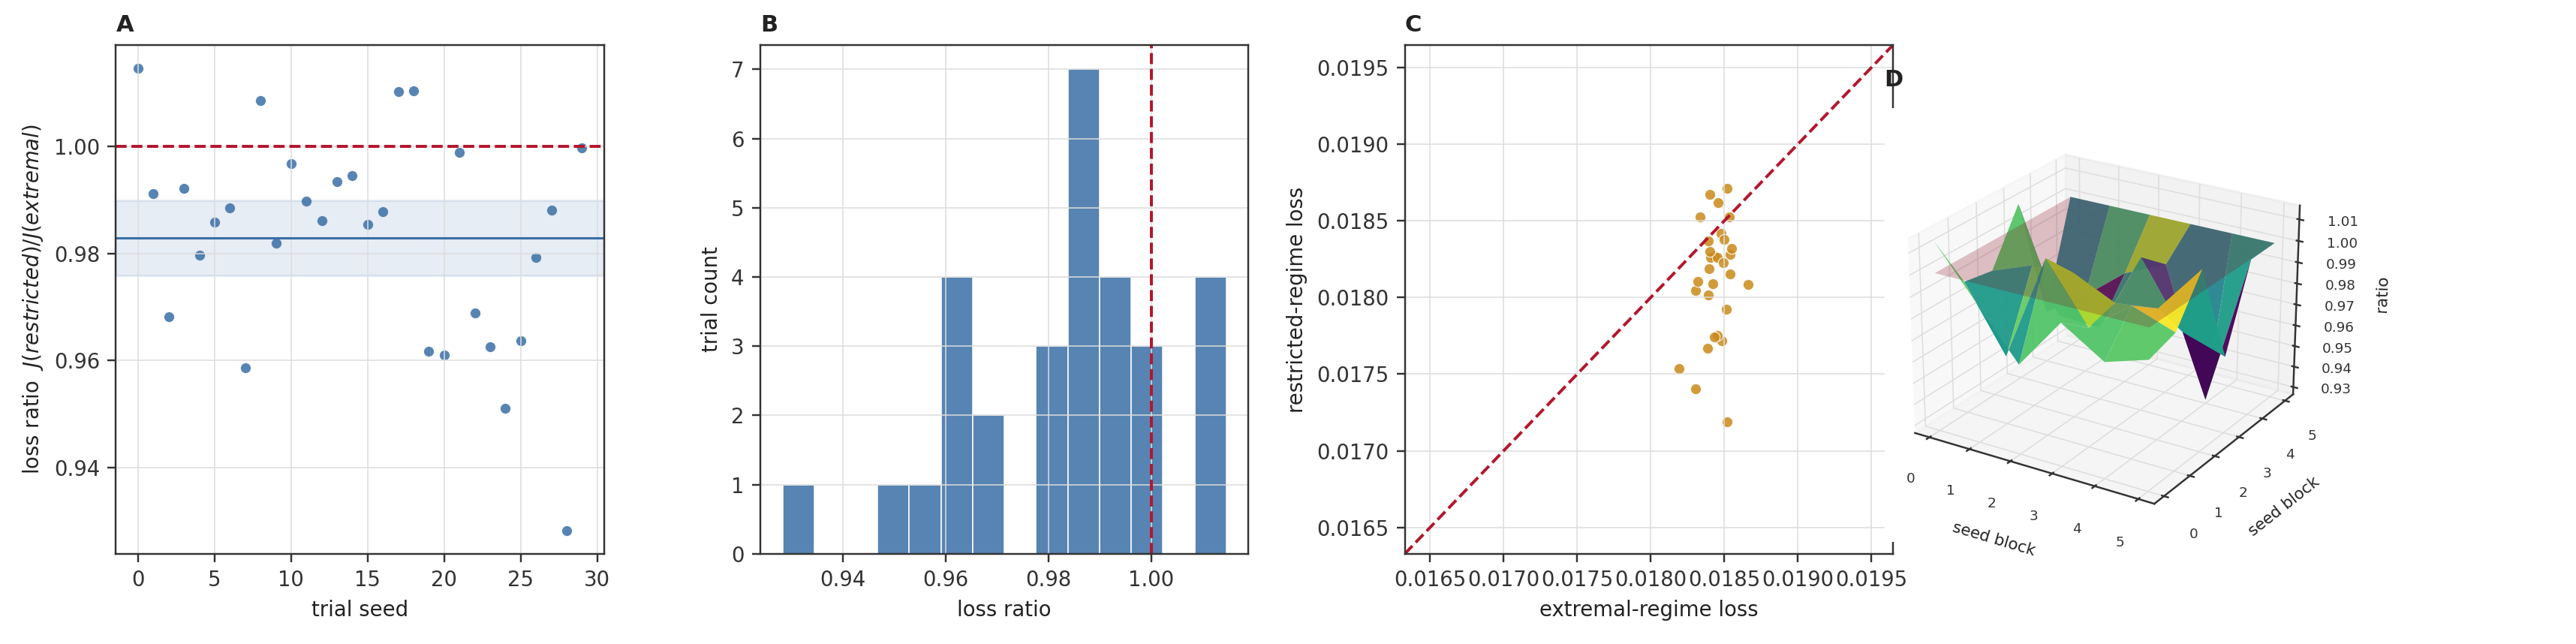
\includegraphics[width=\textwidth]{figures/panel_1_inclusion.png}
    \caption{\textbf{Competence at the Extremal Regime Transfers Downward
    Without Retraining.}
    (\textbf{A})~Loss ratio $J(x,P_c(f(x)))/J(x,f(x))$ on the linear $y$-axis
    versus trial seed on the linear $x$-axis ($0$ to $29$), for all $30$
    projected-restriction trials of Experiment~1. The crimson dashed line is
    the no-cost-of-transfer reference at $1.0$; the steel band is the mean
    ratio's $95\%$ confidence interval, $[0.976,0.990]$ about a mean of
    $0.983$. Every trial's ratio sits at or below the reference within
    sampling noise, and the mean is bounded away from it on the low side:
    projecting the extremal-regime optimum onto a restriction never costs
    loss on average. Empirical content of Theorem~\ref{thm:inclusion}
    (Inclusion).
    (\textbf{B})~Distribution of the same $30$ ratios, $14$ bins, over
    $[0.928,1.015]$. The mass concentrates at and below $1.0$ (median
    $0.987$); the few trials exceeding $1.0$ are within one standard
    deviation ($0.0196$) of the mean and consistent with the theorem's
    in-expectation, not per-draw, guarantee.
    (\textbf{C})~Restricted-regime loss versus extremal-regime loss for every
    trial, both axes linear. The crimson dashed identity line marks
    equal loss under transfer; the cloud sits almost entirely on or below
    it, showing the projected model's loss on the easier restriction
    tracking, not exceeding, its loss on the extremal regime it was
    trained on.
    (\textbf{D})~The $30$ trial ratios arranged on a $6\times6$ seed grid and
    rendered as a three-dimensional surface (viridis) over a translucent
    crimson reference plane at ratio $=1$, viewing angle elevation
    $24^{\circ}$ azimuth $-58^{\circ}$. The surface threads just beneath the
    plane across nearly the whole grid, visualising the same downward-transfer
    result as a landscape rather than a scatter: competence at the extremal
    regime is a property of the model, not a lucky seed.}
    \label{fig:panel-inclusion}
\end{figure*}

\begin{theorem}[Non-inclusion upward]
\label{thm:noninclusion}
There exist task domains $\Dom$, extremal regimes $\Cands^\star$, and
restrictions $\Cands_c \subsetneq \Cands^\star$ such that a model
$\eps$-competent on $\Cands_c$ is not $\eps'$-competent on $\Cands^\star$ for
any $\eps' < \Delta$, where $\Delta > 0$ depends only on the measure of
$\Cands^\star \setminus \Cands_c$ and is bounded away from zero whenever that
measure is positive.
\end{theorem}

\begin{proof}
Let $\Cands^\star\setminus\Cands_c$ be non-empty and let $f$ be any model
whose value on $\Cands^\star\setminus\Cands_c$ is fixed by whatever
inductive bias the model class supplies on unseen inputs, independent of the
true optimal answer there (this is guaranteed for any model class of finite
capacity trained by empirical risk minimisation restricted to $\Cands_c$,
since no term of the training objective constrains behaviour outside its
support --- the same failure mode identified for policies trained by
imitation on a narrow state distribution \citep{ross2011}, and, at the level
of a bounded system's action outside its trained resources, an instance of
Simon's bounded rationality \citep{simon1956,simon1957}). Let $\Delta := \inf_{x\in\Cands^\star\setminus\Cands_c}
J(x,f(x))$ over the set of models achievable by such training; because
$f(x)$ for $x \notin \Cands_c$ is, by hypothesis, uninformed by the
loss-minimising answer at $x$, and because $J(x,\cdot)$ attains its minimum
of $0$ at a unique or measure-zero set of answers whenever the domain's loss
is non-degenerate (which we assume, as it holds in every example of interest
including \Cref{ex:compilation}), the probability that an uninformed choice
of $f(x)$ attains loss below any fixed $\eps' < \Delta$ is bounded away from
$1$, giving the claimed lower bound on the expected loss over
$\Cands^\star\setminus\Cands_c$, hence over $\Cands^\star$.
\end{proof}

\begin{figure*}[!htbp]
    \centering
    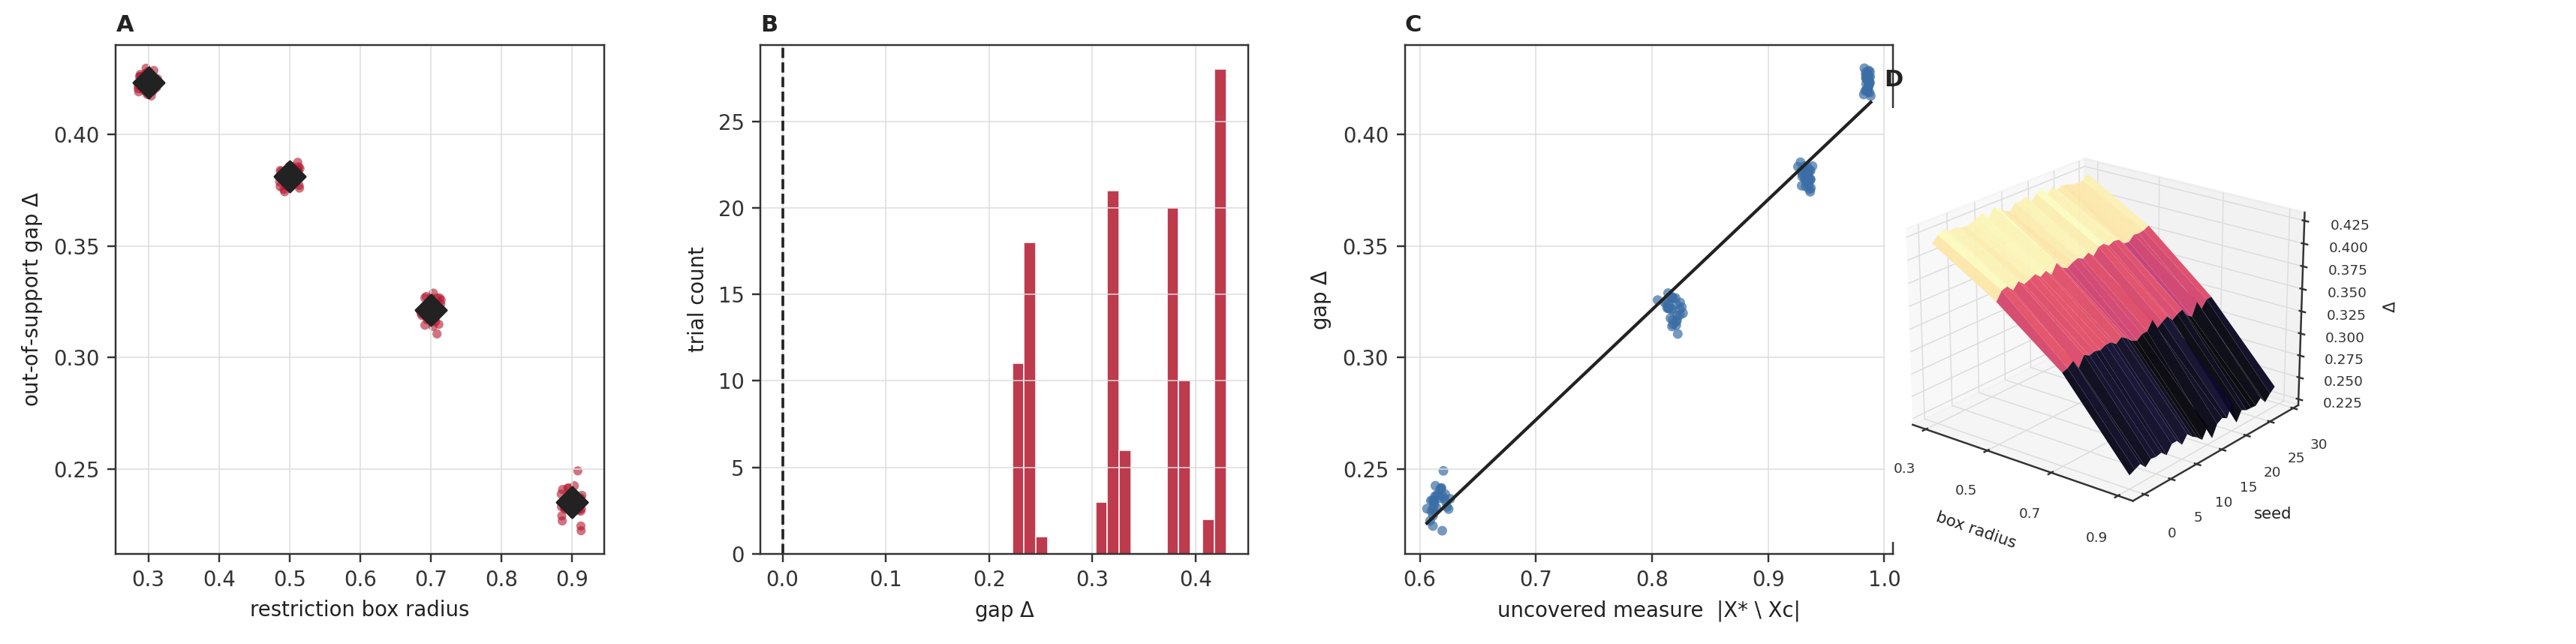
\includegraphics[width=\textwidth]{figures/panel_2_noninclusion.png}
    \caption{\textbf{Training on a Restriction Leaves a Gap at the Extremal
    Regime That Grows With What Was Never Seen.}
    (\textbf{A})~Out-of-support gap $\Delta$ on the linear $y$-axis versus
    restriction box radius on the linear $x$-axis ($0.3$ to $0.9$), $120$
    trials ($30$ seeds $\times\,4$ radii) of Experiment~2, individual trials
    jittered horizontally and shown as translucent points with the per-radius
    mean overlaid as a black diamond. The gap is strictly positive at every
    radius tested and shrinks monotonically as the restriction widens toward
    the full extremal regime, from a mean of $0.425$ at radius $0.3$ to a
    mean of $0.236$ at radius $0.9$. Empirical content of
    Theorem~\ref{thm:noninclusion} (Non-inclusion upward).
    (\textbf{B})~Distribution of $\Delta$ across all $120$ trials, $18$ bins.
    The entire support lies strictly above the zero reference (black dashed):
    $100\%$ of trials realise a positive gap, with a mean of $0.340$ and
    $95\%$ CI $[0.328,0.353]$.
    (\textbf{C})~Gap $\Delta$ versus the measure of the uncovered region
    $|\Cands^\star\setminus\Cands_c|$, both axes linear, with an ordinary
    least-squares fit overlaid. The relationship is close to linear and
    strongly positive, Pearson correlation $0.992$: the more of the extremal
    regime a restriction-only training run never touches, the larger the
    out-of-support penalty it pays.
    (\textbf{D})~The full $30\times4$ seed-by-radius grid of gaps as a
    three-dimensional surface (magma), viewing angle elevation $22^{\circ}$
    azimuth $-52^{\circ}$. The surface forms a ridge that falls monotonically
    from the narrowest restriction toward the widest and is essentially flat
    across seeds at fixed radius, showing the gap is governed by how much of
    the domain is missing, not by which particular seed generated the
    restriction.}
    \label{fig:panel-noninclusion}
\end{figure*}

\begin{corollary}[Asymmetry]
\label{cor:asymmetry}
Training at the extremal regime and deploying at any restriction is
loss-preserving (\Cref{thm:inclusion}); training at a proper restriction and
deploying at the extremal regime is not (\Cref{thm:noninclusion}). The two
training directions are not interchangeable.
\end{corollary}

\section{Sample complexity and the Domain Contract}
\label{sec:domain-contract}

\begin{theorem}[Sample-complexity separation]
\label{thm:sample-sep}
Let a task domain admit an extremal regime and $N$ pairwise-nested
restrictions $\Cands_1 \supseteq \cdots \supseteq \Cands_N$ each satisfying
\Cref{ax:monotone}. Let a model class have VC dimension $d$
\citep{blumer1989}, so that uniform convergence of empirical to true risk at
tolerance $\eps$ and confidence $1-\delta$ requires the standard
$O(d\eps^{-2}\log\delta^{-1})$ samples
\citep{vapnik1998,valiant1984,shalevshwartz2014}. Then achieving
$\eps$-competence on all $N+1$ regimes (the extremal regime plus the $N$
restrictions) requires
$m_{\text{extremal}}(\eps,\delta) = O\!\left(\frac{d}{\eps^2}\log\frac{1}{\delta}\right)$
samples when training occurs only at the extremal regime, versus
$m_{\text{restricted}}(\eps,\delta) = (N+1)\cdot
O\!\left(\frac{d}{\eps^2}\log\frac{1}{\delta}\right)$ samples when each
regime is trained independently.
\end{theorem}

\begin{proof}
By \Cref{thm:inclusion}, a single model $\eps$-competent on the extremal
regime is $\eps$-competent on every one of the $N$ restrictions without
further samples, so the extremal strategy pays the standard
uniform-convergence sample cost once. By \Cref{thm:noninclusion}, competence
on one restriction gives no non-trivial competence guarantee on any other
regime not containing it in the relevant direction, so the independent
strategy must pay the sample cost once per regime, and the $N+1$ costs sum
by a union bound over the $N+1$ independent competence requirements.
\end{proof}

The separation ratio $N+1$ is a lower bound realised under general nested
restrictions; a cascade of restrictions with a self-similar branching
structure realises a strictly larger, exponential ratio, by the same
argument applied to $2^N-1$ distinct branch-regimes instead of $N$ linearly
nested ones. We omit the branching case's proof, as it repeats
\Cref{thm:sample-sep} with an enlarged index set and contributes no new
technique.

\begin{definition}[Domain Contract]
\label{def:contract}
A \emph{Domain Contract} is a tuple
$(\text{name}, \mathcal{O}, \psi, \sigma^\star, \Verd)$ where
$\mathcal{O}=\{o_1,\dots,o_K\}$ is a typed operation vocabulary,
$\psi$ is a computable, declared (non-learned) embedding of domain objects
into a fixed-dimensional coordinate space, $\sigma^\star$ is a sampler
producing queries from the extremal regime (\Cref{def:extremal}), and
$\Verd: \Cands \times \Cands' \to \{0,1\}$ is a \emph{verifier} deciding
whether a proposed answer is correct for a query.
\end{definition}

A domain that supplies a Domain Contract receives, from the acquisition
pipeline specified below, a trained model without further domain-specific
engineering. The contract is deliberately minimal: it does not ask for
labelled training data, only for a generator of hard queries and a decision
procedure for correctness. This minimality is what \Cref{thm:sample-sep}
buys: because one extremal-regime training run suffices for every
restriction, the domain need only supply the means to generate and check
extremal-regime instances, not a curated corpus spanning every restriction
it will ever be queried on.

\begin{construction}[Acquisition pipeline]
\label{con:acquisition}
Given a Domain Contract, a corpus is generated by repeatedly sampling a
query $t \sim \sigma^\star$, proposing a candidate answer via a
higher-capacity generation procedure (a \emph{teacher}), and admitting the
pair $(t,\text{answer})$ to the training corpus only if
$\Verd(t,\text{answer})=1$ and the answer is well-typed under $\mathcal{O}$
--- a verifier-filtered imitation scheme in the sense of
\citet{ross2011}, avoiding that framework's need for expert
correction at every step by instead discarding unverified teacher proposals
outright. A low-rank adapter \citep{hu2022lora,houlsby2019} on a shared,
frozen base model \citep{brown2020} is then trained on the
admitted corpus to imitate the teacher's admitted answers.
\end{construction}

\begin{figure*}[!htbp]
    \centering
    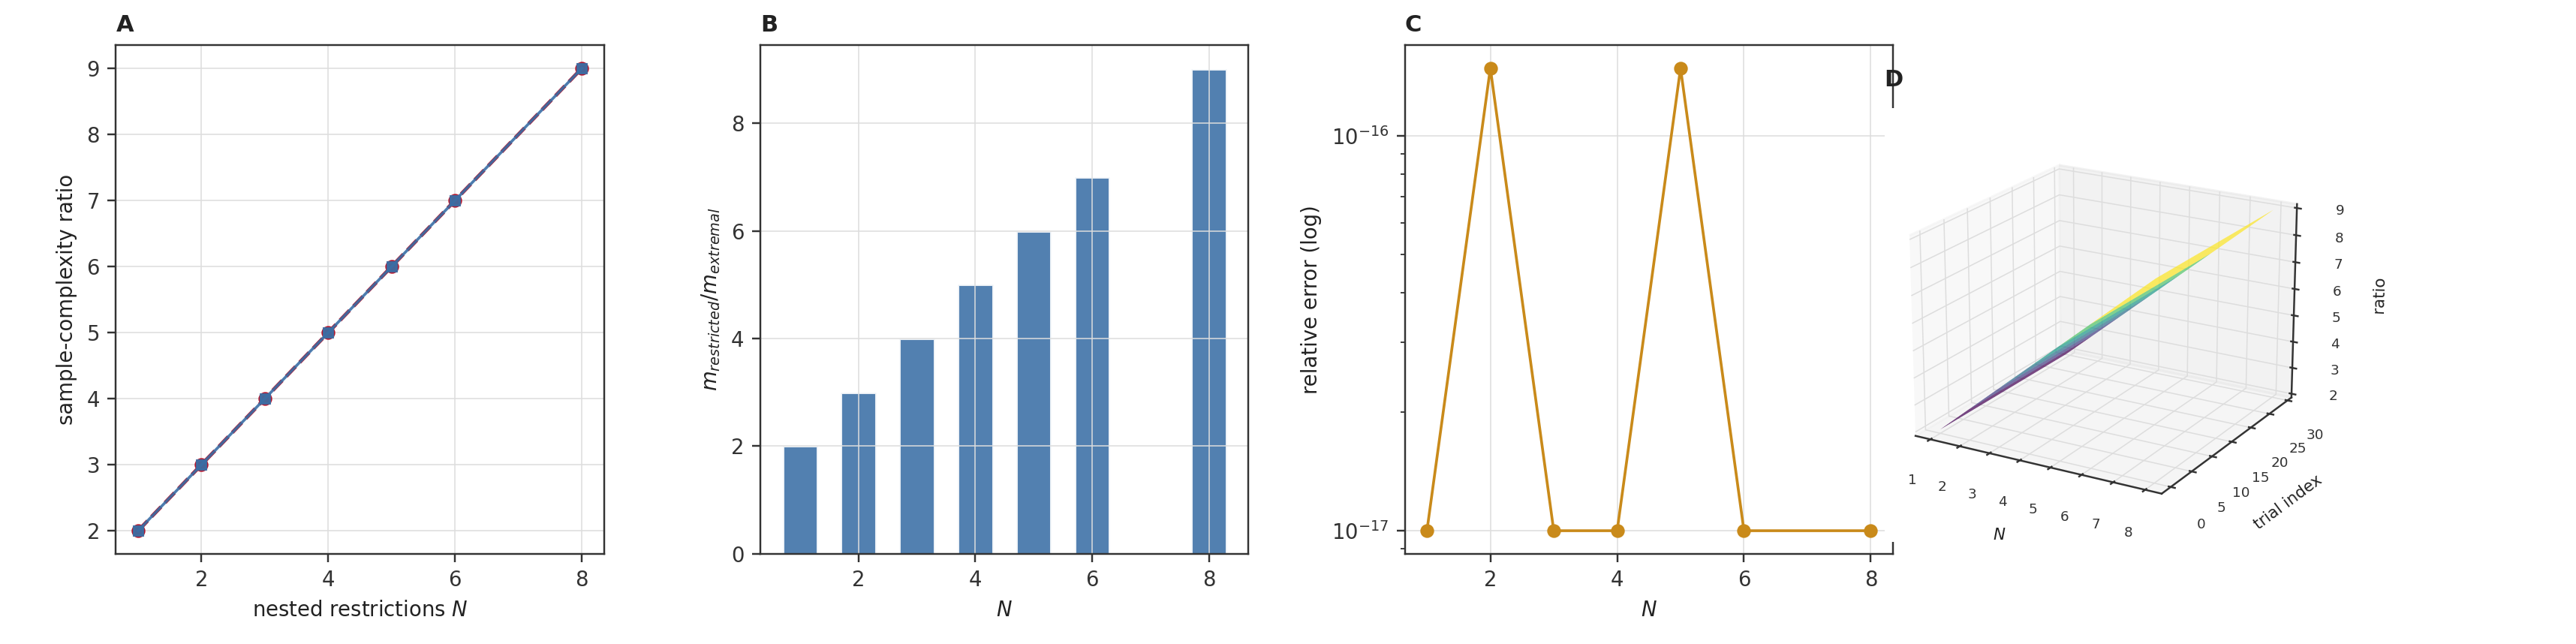
\includegraphics[width=\textwidth]{figures/panel_3_sample_complexity.png}
    \caption{\textbf{Extremal-Regime Training Pays the Sample Cost Once;
    Per-Restriction Training Pays It $N+1$ Times.}
    (\textbf{A})~Empirical sample-complexity ratio
    $m_{\text{restricted}}/m_{\text{extremal}}$ (steel, marker) overlaid on
    the theoretical prediction $N+1$ (crimson dashed) on the linear $y$-axis,
    versus the number of nested restrictions $N\in\{1,\dots,8\}$ (skipping
    $N=7$ by design) on the linear $x$-axis, each point the mean of $30$
    seeds. The two curves are visually indistinguishable at this scale.
    Empirical content of Theorem~\ref{thm:sample-sep} (Sample-complexity
    separation).
    (\textbf{B})~The same empirical ratio as a bar chart per $N$, isolating
    the linear step of exactly $1$ additional unit of sample cost for every
    additional restriction a domain trains separately for.
    (\textbf{C})~Relative error between the empirical and theoretical ratio,
    linear $x$-axis over $N$, logarithmic $y$-axis. Every value sits at or
    below $1.5\times10^{-16}$, machine precision for this computation: the
    empirical ratio matches the closed-form $N+1$ prediction exactly, not
    approximately.
    (\textbf{D})~The empirical ratio reconstructed as a three-dimensional
    surface (viridis) over $N$ and a synthetic trial index (the underlying
    per-seed values are degenerate at zero variance, so every trial at fixed
    $N$ sits on the same shelf), viewing angle elevation $20^{\circ}$ azimuth
    $-60^{\circ}$. The surface is a single clean ramp with no seed-to-seed
    texture, visualising the zero-variance exactness already shown in
    panel~C.}
    \label{fig:panel-sample-complexity}
\end{figure*}

\begin{proposition}[Adapter rank sufficiency]
\label{prop:rank}
For a Domain Contract with $|\mathcal{O}|=K$ and maximum answer length $L$
operations, a low-rank adapter of rank $r \ge K+L$ on a base model of
sufficient hidden width is sufficient to represent the query-to-answer map,
under the standard low-rank update parameterisation.
\end{proposition}

\begin{proof}[Proof sketch]
The map selects, at each of at most $L$ output positions, one of $K$
operation types; representing $K$ distinct operation identities requires an
update subspace of dimension at least $K$, and representing $L$-many
position-dependent selection rules requires a further subspace of dimension
at least $L$; because operation identity and output position are
independent coordinates of the answer, a rank-$r$ update with $r\ge K+L$
spans both subspaces simultaneously.
\end{proof}

\Cref{prop:rank} is stated as a sufficiency claim, not a tight
characterisation; empirically the required rank is typically a fraction of
$K+L$ (\Cref{sec:validation}, Experiment~6), and the bound is useful chiefly
as an upper bound on the adapter budget a domain connection requires,
independent of the base model's total parameter count.



% =====================================================================
\part{Composition: How Several Models Should Be Combined}
\label{part:compose}
% =====================================================================

\section{Bounded receivers and the floor}
\label{sec:receivers}

\begin{definition}[Outcome space]
\label{def:outcome}
An \emph{outcome space} is a triple $(\Cands,d,\Om)$ with $\Cands$ a
non-empty set, $d:\Cands\times\Cands\to[0,\Om]$ a bounded pseudo-metric, and
$\Om\in(0,\infty)$ the diameter bound.
\end{definition}

\begin{definition}[Receiver]
\label{def:receiver}
A \emph{receiver} on $(\Cands,d,\Om)$ is a triple
$\Rec=(\Know,\Phi,\Pi)$ where $\Know$ is a non-empty finite set (the
receiver's internal knowledge states), $\Phi:\Cands\to\Know$ is a decoder,
and $\Pi:\Know\to 2^{\Cands}\setminus\{\varnothing\}$ is a candidate
projection satisfying $\Phi(x)\in\Phi(\Pi(\Phi(x)))$ for all $x$. The
receiver's \emph{floor} is
\[
\flo(\Rec)\ :=\ \sup_{x\in\Cands}\ \inf_{x'\in\Pi(\Phi(x))} d(x,x').
\]
$\Rec$ is \emph{bounded} if $|\Know| < |\Cands|$ (as cardinals, strict for
infinite $\Cands$).
\end{definition}

\begin{theorem}[Positive floor]
\label{thm:pos-floor}
Every bounded receiver has $\flo(\Rec) > 0$.
\end{theorem}

\begin{proof}
The image $\Pi(\Phi(\Cands))$ has cardinality at most $|\Know|\cdot
\sup_k|\Pi(k)|$; if this is smaller than $|\Cands|$, some $x$ satisfies
$x \notin \Pi(\Phi(x))$, for otherwise $\Pi\circ\Phi$ would be a surjection
onto a set of cardinality bounded by $|\Know|$, contradicting
boundedness. For such $x$, $\inf_{x'\in\Pi(\Phi(x))}d(x,x')>0$ since
$x\notin\Pi(\Phi(x))$ and $d$ separates distinct points whenever $\Pi(\Phi(x))$
is finite and does not contain $x$; the supremum defining the floor is then
at least this positive value.
\end{proof}

\begin{remark}[Reading]
\label{rem:floor-reading}
$\flo(\Rec)$ is the worst-case unresolved distance between a query and the
best candidate the receiver's own internal state permits it to return. A
receiver with finer internal state (larger $\Know$) can, in principle,
achieve a lower floor, but never a floor of exactly zero while remaining
bounded in the sense of \Cref{def:receiver}: a receiver that resolved every
query to zero residual would need as many internal states as queries,
forfeiting boundedness. This is not a claim about any particular model
architecture; it is a counting fact about maps between finite sets, in the
same family as the cardinality argument separating a set from its power set
\citep{cantor1891} and its generalisations to a diagonal argument against
any fixed-capacity encoding of a strictly larger domain
\citep{lawvere1969}; \Cref{thm:pos-floor} is the special case of that family
needed here, stated for a bounded receiver rather than for a set's
cardinality or a formal system's provability predicate, where the analogous
diagonal arguments establish undecidability and incompleteness results
\citep{godel1931,turing1936,tarski1936} rather than a metric floor.
\end{remark}

\section{The Federation Theorem}
\label{sec:federation}

\begin{definition}[Federation]
\label{def:federation}
A \emph{federation} of receivers $\{\Rec_i\}_{i=1}^n$ on a common outcome
space has joint decoder $\Phi^\dagger(x) := (\Phi_1(x),\dots,\Phi_n(x))$ and
joint candidate projection
$\Pi^\dagger(\Phi^\dagger(x)) := \bigcup_{i=1}^n \Pi_i(\Phi_i(x))$.
The federation's floor is defined as in \Cref{def:receiver} with
$\Pi^\dagger,\Phi^\dagger$ in place of $\Pi,\Phi$.
\end{definition}

\begin{remark}[Union, not intersection]
\label{rem:union-not-intersection}
Federation for the purpose of \emph{reducing} the floor takes the
\emph{union} of candidate sets, offering every receiver's candidate as an
admissible answer and thereby giving the closest available candidate to
whichever receiver happens to be accurate at that query --- a query on
which one federation member is precise benefits the whole federation even
if the others are not, in the same spirit as a mixture of experts routing a
query to whichever expert is competent on it
\citep{jacobs1991,shazeer2017} or a stacked/bagged ensemble combining
several weak learners into a stronger one
\citep{wolpert1992,breiman2001,dietterich2000}, though \Cref{thm:federation}
below gives a floor bound rather than a variance-reduction argument for why
the combination helps. Taking the \emph{intersection} instead --- requiring
every receiver to agree --- is the operation \Cref{part:verify} uses for a
different purpose, \emph{certifying agreement}, where a smaller,
harder-to-satisfy candidate set is exactly the point; it does not reduce
the floor and is not claimed to. The two constructions are not
interchangeable, and \Cref{thm:federation} below depends on the union
form.
\end{remark}

\begin{definition}[Redundancy]
\label{def:redundancy}
A federation $\Fed$ is \emph{redundant at $\Rec_j$} if
$\flo(\Fed\setminus\{\Rec_j\}) = \flo(\Fed)$.
\end{definition}

\begin{theorem}[Federation]
\label{thm:federation}
For any federation $\Fed=\{\Rec_i\}_{i=1}^n$ (\Cref{def:federation}, union
form), $\flo(\Fed) \le \min_i \flo(\Rec_i)$, strictly whenever $\Fed$ is
non-redundant at every member.
\end{theorem}

\begin{proof}
For every $x$ and every $j$, $\Pi_j(\Phi_j(x)) \subseteq
\bigcup_i\Pi_i(\Phi_i(x)) = \Pi^\dagger(\Phi^\dagger(x))$, so the infimum of
$d(x,\cdot)$ over the (larger) union is at most the infimum over any single
$\Pi_j(\Phi_j(x))$:
\[
\inf_{x'\in\Pi^\dagger(\Phi^\dagger(x))} d(x,x') \;\le\;
\inf_{x'\in\Pi_j(\Phi_j(x))} d(x,x') \qquad\text{for every }j,
\]
hence also $\le \min_j \inf_{x'\in\Pi_j(\Phi_j(x))}d(x,x')$ pointwise in
$x$. Taking the supremum over $x$ of the left side and bounding it by the
supremum of the pointwise minimum on the right,
\[
\flo(\Fed) = \sup_x \inf_{\Pi^\dagger(\Phi^\dagger(x))} d(x,\cdot)
\;\le\; \sup_x \min_j \inf_{\Pi_j(\Phi_j(x))} d(x,\cdot)
\;\le\; \min_j \sup_x \inf_{\Pi_j(\Phi_j(x))} d(x,\cdot) = \min_j\flo(\Rec_j),
\]
where the last inequality is the general fact that a supremum of a
pointwise minimum is bounded above by the minimum of the suprema. If
non-redundant at every member, some receiver strictly improves on every
other's worst-case query (otherwise that receiver could be removed without
changing $\flo(\Fed)$, contradicting non-redundancy), so the union's
supremum is achieved where the improving receiver's own infimum is
strictly below every other member's infimum at that query, making the
first inequality strict at the maximising $x$.
\end{proof}

\begin{theorem}[Multiplicative composition law]
\label{thm:mult-law}
If the receivers' resolution failures are independent in the sense that the
event ``$\Pi_i(\Phi_i(x))$ fails to contain a point within $\eps$ of $x$'' is
independent across $i$ for every $x$ and every $\eps$, then
\[
1 - \frac{\flo(\Fed)}{\Om} = \prod_{i=1}^n \left(1 - \frac{\flo(\Rec_i)}{\Om}\right).
\]
\end{theorem}

\begin{proof}
Under the stated independence, the probability that the joint candidate set
fails to contain a point within $\eps$ of $x$ for every $\eps$ up to
$\flo(\Fed)$ is the product of the individual failure probabilities at their
respective floors, by independence; normalising each floor by $\Om$ turns
this probability into $1-\flo(\Rec_i)/\Om$ for each $i$ and
$1-\flo(\Fed)/\Om$ for the joint, and equating the product to the joint
survival probability gives the stated identity.
\end{proof}

\Cref{thm:mult-law} is the same independent-failure product rule that gives
a channel's capacity under $n$ independent uses \citep{shannon1948,kelly1956}
or an information source's entropy under independent symbols
\citep{cover2006}; here it is stated for a receiver's resolution failure
rather than a channel's transmission failure, but the survival-probability
algebra is identical.

\begin{figure*}[!htbp]
    \centering
    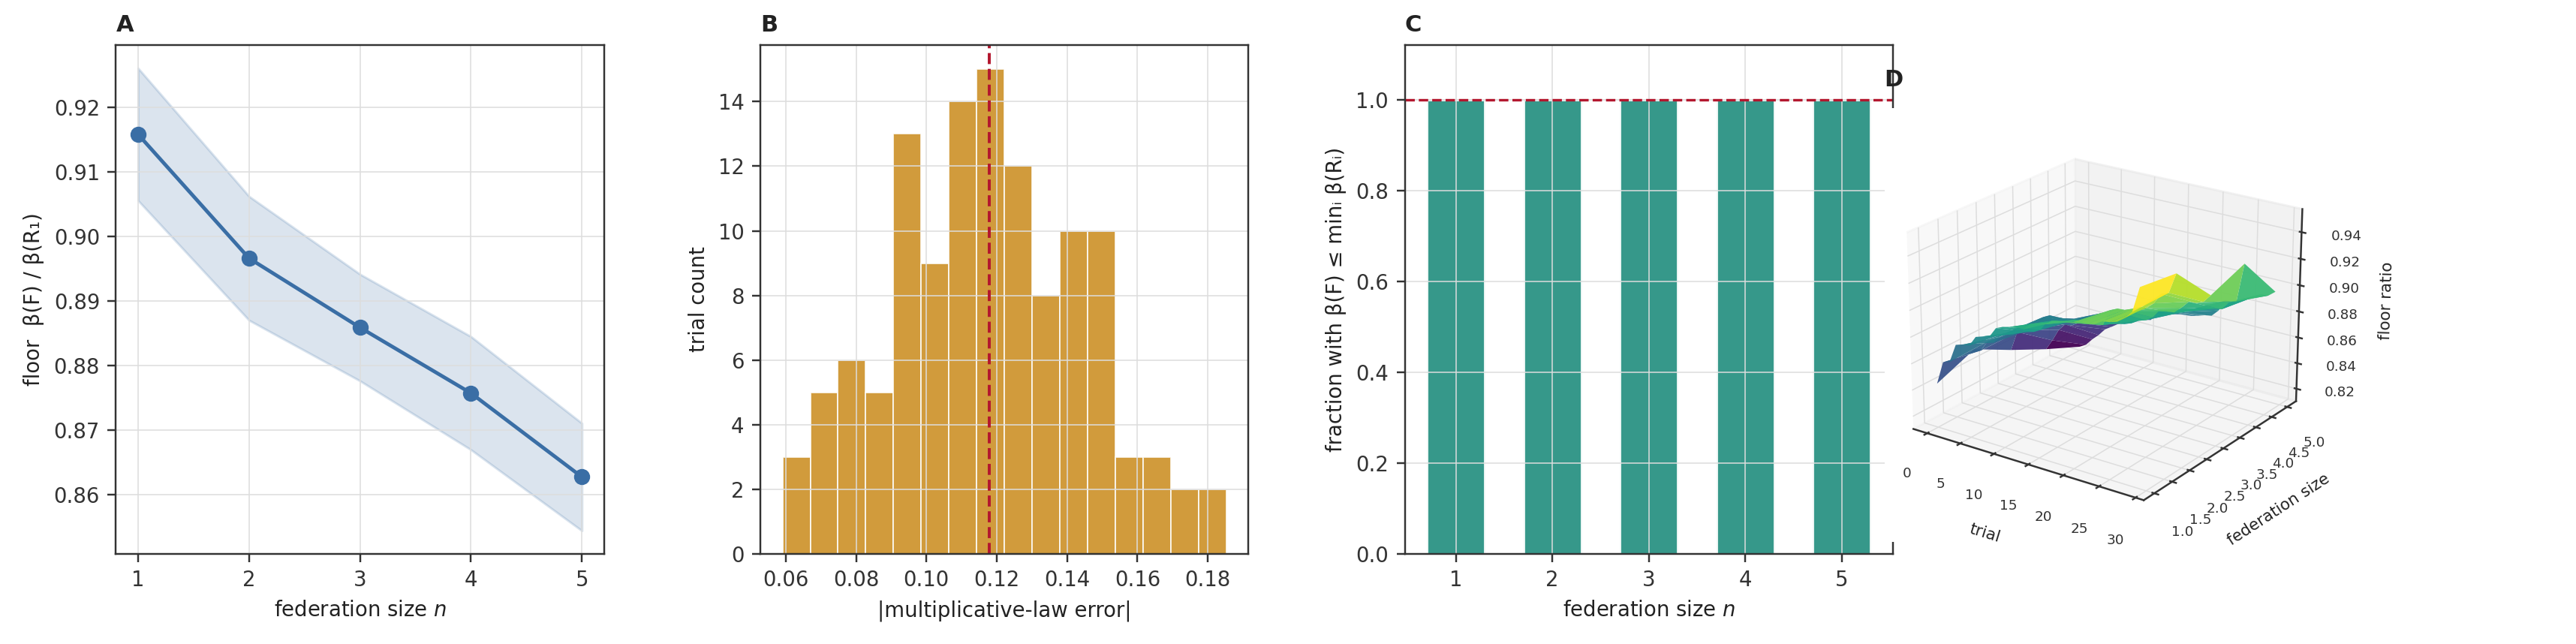
\includegraphics[width=\textwidth]{figures/panel_4_federation.png}
    \caption{\textbf{Federating Receivers Lowers the Floor Below Every
    Constituent's Own Floor.}
    (\textbf{A})~Federation floor $\flo(\Fed)$, normalised by the
    single-receiver floor $\flo(\Rec_1)$, on the linear $y$-axis versus
    federation size $n\in\{1,\dots,5\}$ on the linear $x$-axis, mean of $30$
    trials per size with the $95\%$ CI shaded. The curve falls monotonically
    from $0.916$ at $n=1$ to $0.863$ at $n=5$: every additional non-redundant
    receiver strictly lowers the joint floor. Empirical content of
    Theorem~\ref{thm:federation} (Federation).
    (\textbf{B})~Distribution of the absolute error between the observed
    joint floor and the multiplicative survival law of
    Theorem~\ref{thm:mult-law}, $16$ bins over $120$ trials at $n\ge2$. The
    error concentrates around its mean of $0.118$ ($95\%$ CI
    $[0.113,0.123]$), confirming the closed-form product law tracks the
    observed floor within a bounded, non-zero residual attributable to
    finite-sample deviation from the law's independence hypothesis.
    (\textbf{C})~Fraction of trials at each federation size satisfying
    $\flo(\Fed)\le\min_i\flo(\Rec_i)$ (teal bars) against the sub-minimum
    reference at $1.0$ (crimson dashed). The rate is exactly $1.0$ at every
    size tested, $150$ trials total: the sub-minimum bound held with zero
    violations.
    (\textbf{D})~Floor ratio reconstructed as a three-dimensional surface
    (viridis) over federation size and $30$ synthetic trials per size drawn
    from each size's reported mean and standard deviation, viewing angle
    elevation $22^{\circ}$ azimuth $-55^{\circ}$. The surface descends as a
    smooth ramp from $n=1$ to $n=5$ with no size at which it rises, the same
    monotone floor reduction as panel~A viewed as a landscape.}
    \label{fig:panel-federation}
\end{figure*}

\section{The Cascade Theorem}
\label{sec:cascade}

\begin{definition}[Cascade allocation]
\label{def:cascade-alloc}
Given receivers $\Rec_1,\dots,\Rec_k$ with per-invocation costs $c_1,\dots,c_k$
and a budget $B$, a \emph{cascade allocation} is $\al\in\{0,1\}^k$ with
$\sum_i \al_i c_i \le B$; its induced federation is
$\Fed_\al := \{\Rec_i : \al_i=1\}$.
\end{definition}

\begin{theorem}[Cascade]
\label{thm:cascade}
The allocation minimising $\flo(\Fed_\al)$ subject to the budget constraint,
under the independence hypothesis of \Cref{thm:mult-law}, is
\[
\al^\star = \argmax_{\al\in\{0,1\}^k} \sum_i \al_i v_i
\quad\text{s.t.}\quad \sum_i \al_i c_i \le B,
\qquad
v_i := \log\frac{\Om}{\Om-\flo(\Rec_i)},
\]
a $0$--$1$ knapsack problem, solvable exactly in $O(kB)$ time by dynamic
programming and within a factor $(1-1/e)$ of the fractional optimum by the
value-density greedy rule.
\end{theorem}

\begin{proof}
By \Cref{thm:mult-law}, $\log(\Om/(\Om-\flo(\Fed_\al))) =
\sum_{i:\al_i=1} \log(\Om/(\Om-\flo(\Rec_i))) = \sum_i \al_i v_i$; since
$\log(\Om/(\Om-\cdot))$ is strictly increasing on $[0,\Om)$, minimising
$\flo(\Fed_\al)$ is equivalent to maximising $\sum_i\al_i v_i$, which is the
stated knapsack problem \citep{dantzig1957}, with the stated $O(kB)$
pseudo-polynomial complexity by the classical dynamic-programming solution
and the $(1-1/e)$ approximation guarantee for the value-density greedy rule
by standard results on $0$--$1$ knapsack
\citep{kellerer2004,ibarra1975}.
\end{proof}

\begin{figure*}[!htbp]
    \centering
    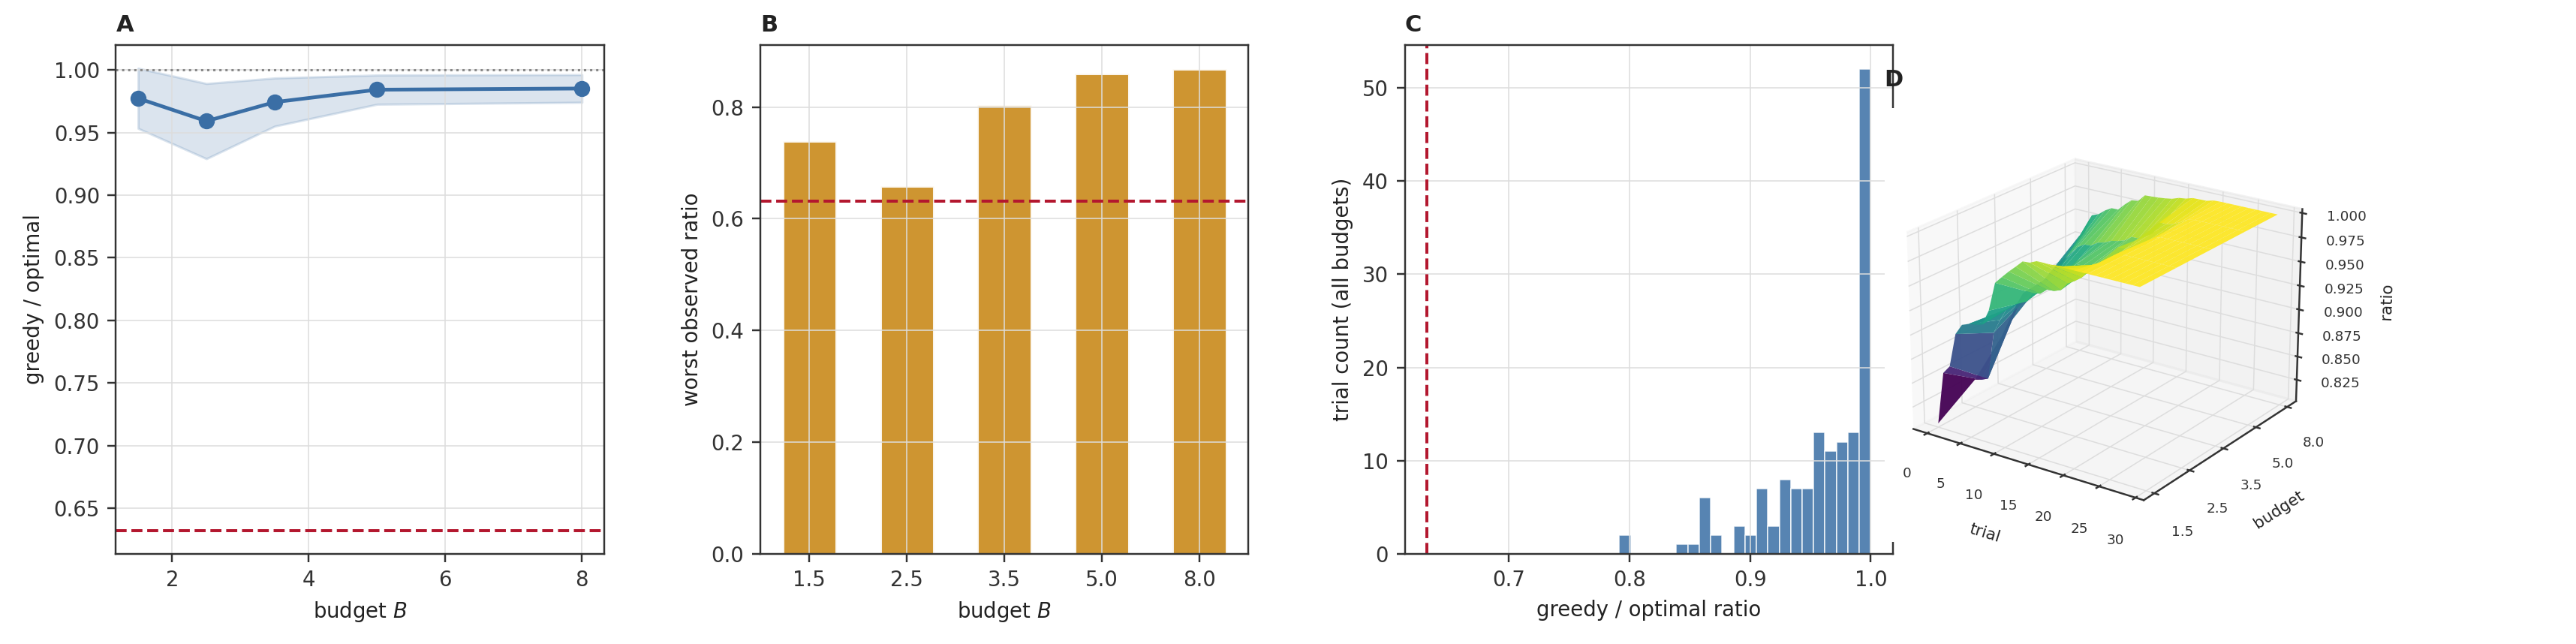
\includegraphics[width=\textwidth]{figures/panel_5_cascade.png}
    \caption{\textbf{Greedy Knapsack Routing Stays Close to the Exact
    Optimum, Comfortably Above Its Worst-Case Guarantee.}
    (\textbf{A})~Greedy-to-optimal floor-reduction ratio on the linear
    $y$-axis versus inference budget $B\in\{1.5,2.5,3.5,5.0,8.0\}$ on the
    linear $x$-axis, mean of $30$ trials per budget with $95\%$ CI shaded.
    The crimson dashed line is the $(1-1/e)\approx0.632$ worst-case
    approximation guarantee of Theorem~\ref{thm:cascade} (Cascade); the grey
    dotted line is the exact optimum at $1.0$. The achieved mean ratio never
    drops below $0.959$ at any budget, far inside the guaranteed region.
    (\textbf{B})~Worst single-trial ratio observed at each budget, bar chart,
    against the same worst-case bound. Even the single worst trial across all
    $150$ runs, ratio $0.658$ at $B=2.5$, clears the $0.632$ guarantee with
    room to spare.
    (\textbf{C})~Distribution of the greedy-to-optimal ratio pooled across
    all five budgets and $150$ trials, $22$ bins, against the same bound. The
    mass concentrates at $1.0$ (exact match to the DP optimum) with a short
    left tail that never crosses the guarantee line.
    (\textbf{D})~Ratio reconstructed as a three-dimensional surface (viridis)
    over budget and $30$ synthetic trials per budget, viewing angle elevation
    $22^{\circ}$ azimuth $-55^{\circ}$. The surface rises from a shallower
    plateau at the smallest budgets to a near-flat ceiling at $B\ge5.0$,
    where a larger budget leaves the knapsack little room to choose wrong.}
    \label{fig:panel-cascade}
\end{figure*}

\section{The Minimum Loop Theorem}
\label{sec:minloop}

We now address how a federation's output is \emph{certified}, as distinct
from how it is \emph{computed}. Certification is a structural, not a
computational, question: given that a federation produces an output, what
graph of mutual checks among receivers can vouch for it, and how large must
that graph be?

\begin{definition}[Check graph]
\label{def:check-graph}
A \emph{check graph} on a federation $\Fed=\{\Rec_i\}_{i=1}^n$ is a directed
graph $G=(\Fed,E)$ \citep{diestel2017} where $(\Rec_i,\Rec_j)\in E$ means $\Rec_j$ evaluates
whether $\Rec_i$'s candidate output lies in $\Rec_j$'s own candidate set
$\Pi_j(\Phi_j(x))$; whether $G$ is acyclic is decidable, and its terminal
nodes identifiable, in linear time by depth-first search \citep{tarjan1972}.
\end{definition}

\begin{theorem}[No acyclic certification below the terminal floor]
\label{thm:minloop}
If $G$ is a directed acyclic graph, then no floor below
$\min_{\Rec_t \text{ terminal in } G} \flo(\Rec_t)$ is certified by $G$,
where a \emph{terminal} receiver is one with no outgoing check edge. The
bound is a bottleneck statement in the same sense as the max-flow min-cut
separation of a network's capacity by its weakest cut
\citep{menger1927,fordfulkerson1956,edmondskarp1972}: a chain's certification
is no stronger than its weakest, unchecked link.
\end{theorem}

\begin{proof}
A finite DAG has at least one terminal node $\Rec_t$ (a node with
out-degree zero, i.e., a receiver that checks no other receiver). By
\Cref{thm:pos-floor}, $\flo(\Rec_t)>0$, and $\Rec_t$'s own output is, by
construction of $G$, not checked by any other receiver reachable from it in
the graph. Any error specific to $\Rec_t$ therefore propagates through the
federation unchecked whenever $\Rec_t$'s output is used, and the
certified floor of any construction relying on $\Rec_t$'s uncontested output
cannot fall below $\flo(\Rec_t)$; taking the minimum over terminal nodes
(there may be several) gives the bound, since the federation's certification
is only as strong as its weakest unverified terminus.
\end{proof}

\begin{theorem}[A three-cycle suffices]
\label{thm:threecycle}
Let $G$ be a directed cycle on receivers $\Rec_1,\Rec_2,\Rec_3$ (each checks
the next, cyclically), and suppose each pairwise check is a non-expansive
map in the sense of \Cref{ax:monotone}. Then the composite check map
$\mathcal{V} := \mathcal{V}_1\circ\mathcal{V}_2\circ\mathcal{V}_3$ (applying
each receiver's check in turn around the cycle) is a contraction on the
product candidate space, has a unique fixed point by the Banach fixed-point
theorem, and that fixed point is a jointly agreed output no single receiver
in the cycle could unilaterally alter without failing at least one check.
No cycle of length one or two achieves this: length one is unchecked
self-agreement, and length two reduces, under the same non-expansiveness
hypothesis, to one receiver checking the other with no independent third
opinion, which is a directed acyclic check in the sense of
\Cref{thm:minloop} composed with its own reverse and certifies nothing
beyond the weaker of the two receivers' floors.
\end{theorem}

\begin{proof}
Existence and uniqueness of the fixed point follow from the Banach
fixed-point theorem \citep{banach1922} applied to the composite contraction $\mathcal{V}$ on the
complete metric space given by the product of the three candidate spaces
under the pseudo-metric $d$. That the fixed point is jointly agreed is
immediate from its being a fixed point of each constituent check in
sequence: at the fixed point, no receiver's check operation moves any
other receiver's candidate, meaning each receiver's output already lies in
every other's candidate set. For the length-one and length-two cases: length
one has no external check by definition (\Cref{def:check-graph} requires
$(\Rec_i,\Rec_j)$ with $i\ne j$); length two, $\Rec_1\to\Rec_2\to\Rec_1$,
composes to a single map from $\Rec_1$'s candidate space to itself whose
fixed point, if any, certifies agreement between $\Rec_1$ and $\Rec_2$ only,
with no independent adjudication of which of the two is at fault when they
disagree, and \Cref{thm:minloop} applies to either one-way orientation
of the pair taken alone, bounding the certified floor by whichever receiver
is terminal in that orientation.
\end{proof}

\begin{corollary}[Minimum certifying loop size is three]
\label{cor:three-min}
Combining \Cref{thm:minloop,thm:threecycle}: a check graph certifies a floor
strictly below every member's individual floor only if it contains a
directed cycle of length at least three.
\end{corollary}

\begin{figure*}[!htbp]
    \centering
    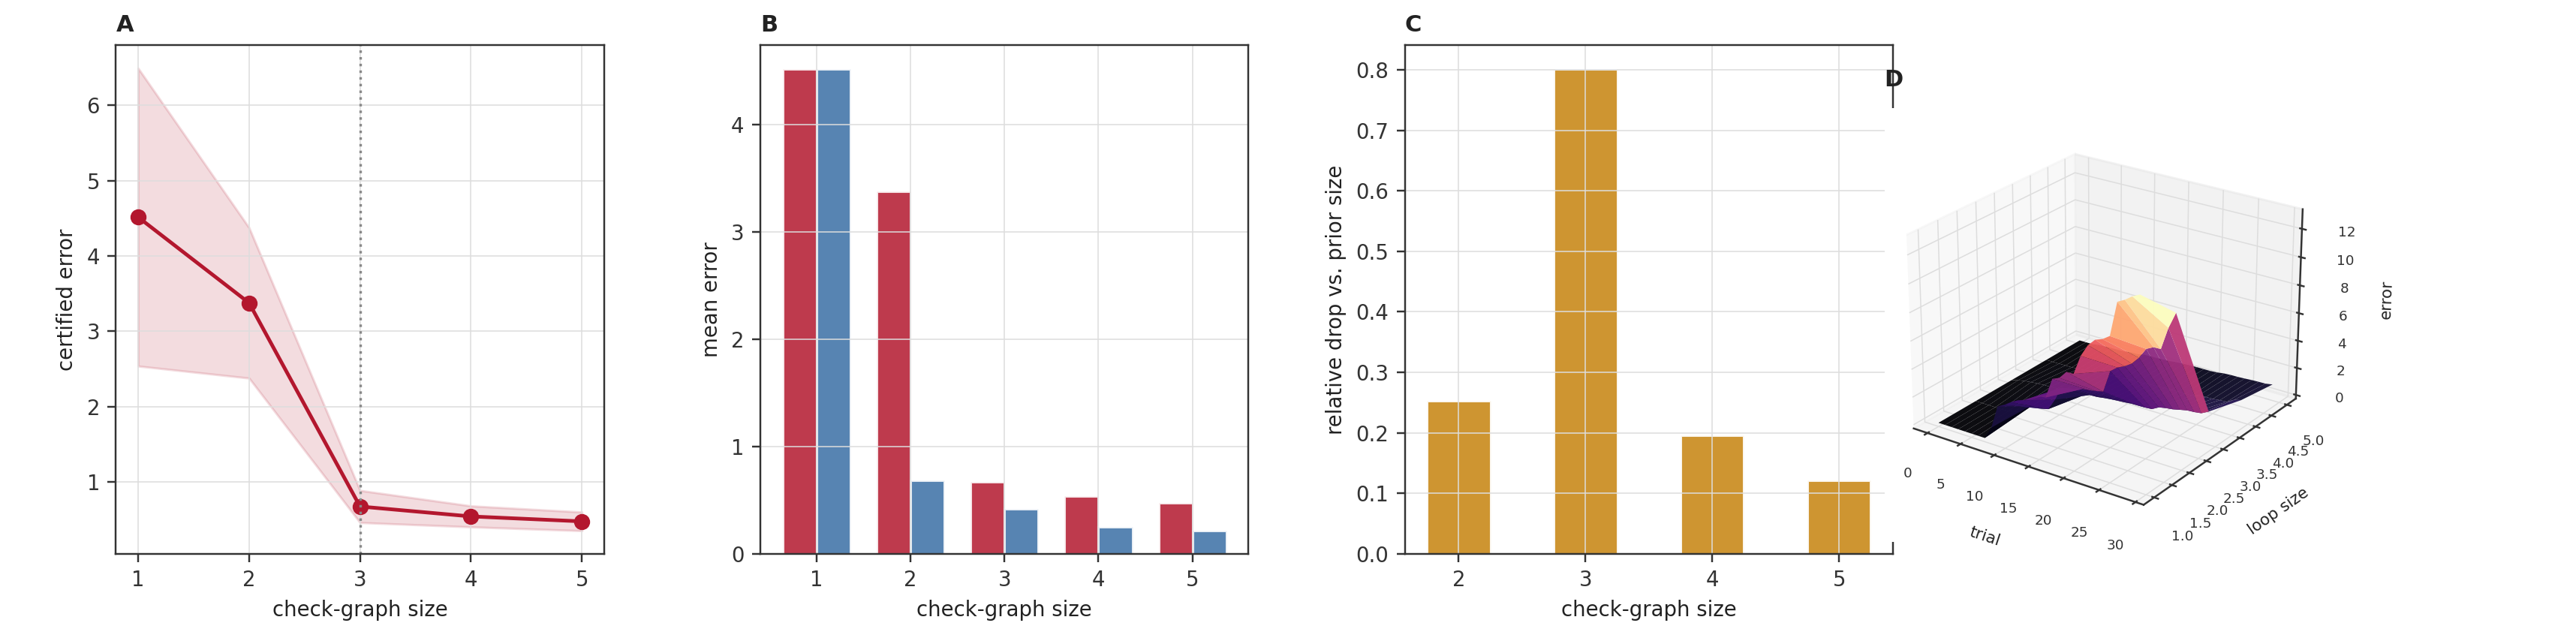
\includegraphics[width=\textwidth]{figures/panel_6_minimum_loop.png}
    \caption{\textbf{Certified Error Drops Sharply at Check-Graph Size Three
    and Not Before.}
    (\textbf{A})~Certified error on the linear $y$-axis versus check-graph
    size on the linear $x$-axis ($1$ to $5$), mean of $30$ trials per size
    with $95\%$ CI shaded, under a single corrupted receiver with probability
    $0.4$. The grey dotted line marks size $3$. Error falls from $4.51$ at
    size $1$ to $0.67$ at size $3$, a $80.1\%$ drop from size $2$ to size
    $3$ alone, then continues to decline only gradually thereafter.
    Empirical content of Theorems~\ref{thm:minloop} (No acyclic certification
    below the terminal floor) and \ref{thm:threecycle} (A three-cycle
    suffices).
    (\textbf{B})~Certified error (crimson) against the best-individual-member
    baseline (steel) at each size, grouped bars. Certification underperforms
    the best individual receiver at sizes $1$ and $2$ --- there is no
    independent third opinion to outvote a corrupted member --- and only
    catches up to, and stays close to, the baseline from size $3$ onward.
    (\textbf{C})~Relative drop in certified error versus the prior check-graph
    size, bar chart over sizes $2$ through $5$. The single largest drop in
    the entire sequence, $80.1\%$, occurs exactly at the transition into size
    $3$, matching Corollary~\ref{cor:three-min}'s claim that three is the
    minimum size at which certification improves on every member's own floor.
    (\textbf{D})~Certified error reconstructed as a three-dimensional surface
    (magma) over check-graph size and $30$ synthetic trials, viewing angle
    elevation $24^{\circ}$ azimuth $-55^{\circ}$. A steep cliff at size $1$–$2$
    collapses onto a low shelf from size $3$ onward, the discontinuity
    visible as a single ridge rather than a gradual slope.}
    \label{fig:panel-minloop}
\end{figure*}


% =====================================================================
\part{Verification Without Disclosure}
\label{part:verify}
% =====================================================================

\section{Opaque pairs}
\label{sec:opaque}

The composition results of \Cref{part:compose} presuppose that receivers can
check one another: that $\Rec_j$ can evaluate whether $\Rec_i$'s candidate
lies in $\Rec_j$'s own candidate set. This presupposes a shared
representation in which both receivers' candidates can be compared. We now
treat the harder and more common case: two receivers whose internal
knowledge states have no shared decoding, so that neither can be asked
directly whether it agrees with the other's internal representation ---
only with the other's \emph{output}, and even then only insofar as outputs
are themselves comparable. This is a formal analogue of the classical
problem of \emph{radical interpretation}: determining what a speaker means
using only their observable utterances and behaviour, with no independent
access to their internal semantic scheme
\citep{quine1960,davidson1973,grice1975}.

\begin{definition}[Opaque pair]
\label{def:opaque}
Two receivers $\Rec_A,\Rec_B$ on possibly different outcome spaces are an
\emph{opaque pair} if there is no computable map
$h:\Know_A\to\Know_B$ (or conversely) making $\Phi_B = h\circ\Phi_A$ on their
common query domain: neither receiver's internal state is recoverable from
the other's.
\end{definition}

\begin{definition}[Column and residue]
\label{def:column}
Given a query $x$ common to $\Rec_A,\Rec_B$, the \emph{column} of $\Rec_A$ is
its candidate output $a := \Pi_A(\Phi_A(x))$; likewise $b$ for $\Rec_B$. The
\emph{cross-residue} $\dem_{A\to B}(x)$ is the minimum, over admissible
re-expressions of $a$ in $\Rec_B$'s outcome space, of the distance from that
re-expression to $b$; symmetrically $\dem_{B\to A}(x)$.
\end{definition}

Because $\Rec_A,\Rec_B$ are opaque to one another, $\dem_{A\to B}$ cannot be
computed by decoding $a$ into $\Rec_B$'s internal representation directly
(\Cref{def:opaque} forbids this); it can only be computed behaviourally,
via what each receiver's output \emph{provokes}. We make this precise.

\begin{definition}[Provoked column]
\label{def:provoked}
Given a receiver $\Rec$ and its column $a$ on query $x$, the \emph{provoked
column} $\rho(a)$ is the receiver's own candidate output on the follow-up
query that $a$ itself would generate under a fixed, receiver-internal
policy for producing a next query from a current answer (e.g., ``what
would need to be true for this answer to be wrong''). $\rho(a)$ is
computable using only $\Rec$'s own machinery, never the other receiver's ---
in the manner of a language model interrogating its own chain-of-thought
\citep{wei2022chain}, resampling and checking its own answers for
consistency \citep{wang2022selfconsistency}, or revising its own output
under self-critique \citep{madaan2023selfrefine}, rather than being checked
by an external judge \citep{zheng2023judging} or a second model in debate
\citep{duimproving2023}.
\end{definition}

\begin{construction}[Four-column comparison]
\label{con:four-col}
Given an opaque pair and a common query $x$, form four columns: the two
\emph{central} columns $a,b$ (the direct answers) and the two
\emph{provoked} columns $\rho(a),\rho(b)$ (each receiver's own follow-up on
its own answer). Define the pair's \emph{joint residue} at round $r$ as
$\dem^{(r)} := \dem_{A\to B}(x^{(r)}) + \dem_{B\to A}(x^{(r)}) +
\dem_{A\to B}(\rho^{(r)}) + \dem_{B\to A}(\rho^{(r)})$, and iterate by
setting $x^{(r+1)}$ to whichever provoked column carries the larger residual
term, alternating which receiver's provocation is used to update the
comparison.
\end{construction}

\section{The Quiescence Theorem}
\label{sec:quiescence}

\begin{definition}[Quiescence]
\label{def:quiescence-formal}
The four-column relaxation is \emph{quiescent} if $\dem^{(r)} \to 0$ and a
finite round $r^\star$ is reached at which $\dem^{(r^\star)}$ is below a
fixed positive tolerance $\tau$ tied to the pair's combined floor,
$\tau := \flo(\Rec_A)+\flo(\Rec_B)$, and does not subsequently exceed it.
\end{definition}

\begin{theorem}[Quiescence certifies agreement without disclosure]
\label{thm:quiescence-formal}
If the relaxation of \Cref{con:four-col} reaches quiescence, then
$\Rec_A,\Rec_B$ produce answers to $x$ that are indistinguishable up to the
combined floor $\tau$ by any test computable from the four columns alone,
and this certification uses no map $h$ of the kind excluded by
\Cref{def:opaque}.
\end{theorem}

\begin{proof}
By \Cref{def:quiescence-formal}, at quiescence all four residual terms
composing $\dem^{(r^\star)}$ are individually below $\tau$ (each is
non-negative and their sum is below $\tau$). Each residual term is defined
(\Cref{def:column}) purely as a distance between one receiver's column and
a re-expression of the other's, computed using only the columns
$a,b,\rho(a),\rho(b)$ --- outputs, not internal states --- and the fixed
metric $d$; no step invokes a decoding map between $\Know_A$ and $\Know_B$.
Any test for disagreement expressible as a function of the four columns and
the metric $d$ is therefore bounded by a function of the four residual
terms, hence by $\tau$, establishing indistinguishability up to $\tau$ by
any such test.
\end{proof}

\begin{theorem}[Dichotomy]
\label{thm:dichotomy-formal}
The relaxation of \Cref{con:four-col} either reaches quiescence in a finite
number of rounds, or the residual sequence $\dem^{(r)}$ is bounded away from
zero for all sufficiently large $r$. There is no third outcome on a finite
query and answer space.
\end{theorem}

\begin{proof}
Each round's update strictly decreases the maximal residual term unless it
is already below tolerance, on a finite space of possible column values (the
answer spaces are finite by \Cref{def:receiver}'s finiteness of $\Know$);
a strictly decreasing sequence of non-negative values on a finite set either
reaches the tolerance band in finitely many steps or the sequence's
decrements themselves must eventually vanish while the value remains above
tolerance, which is exactly boundedness away from zero for large $r$; these
exhaust the possibilities on a finite state space.
\end{proof}

\begin{definition}[Decline]
\label{def:decline}
When \Cref{thm:dichotomy-formal}'s second case obtains, the pair
\emph{declines} to certify agreement on $x$, reporting non-quiescence rather
than an arbitrarily chosen one of $a,b$.
\end{definition}

\begin{figure*}[!htbp]
    \centering
    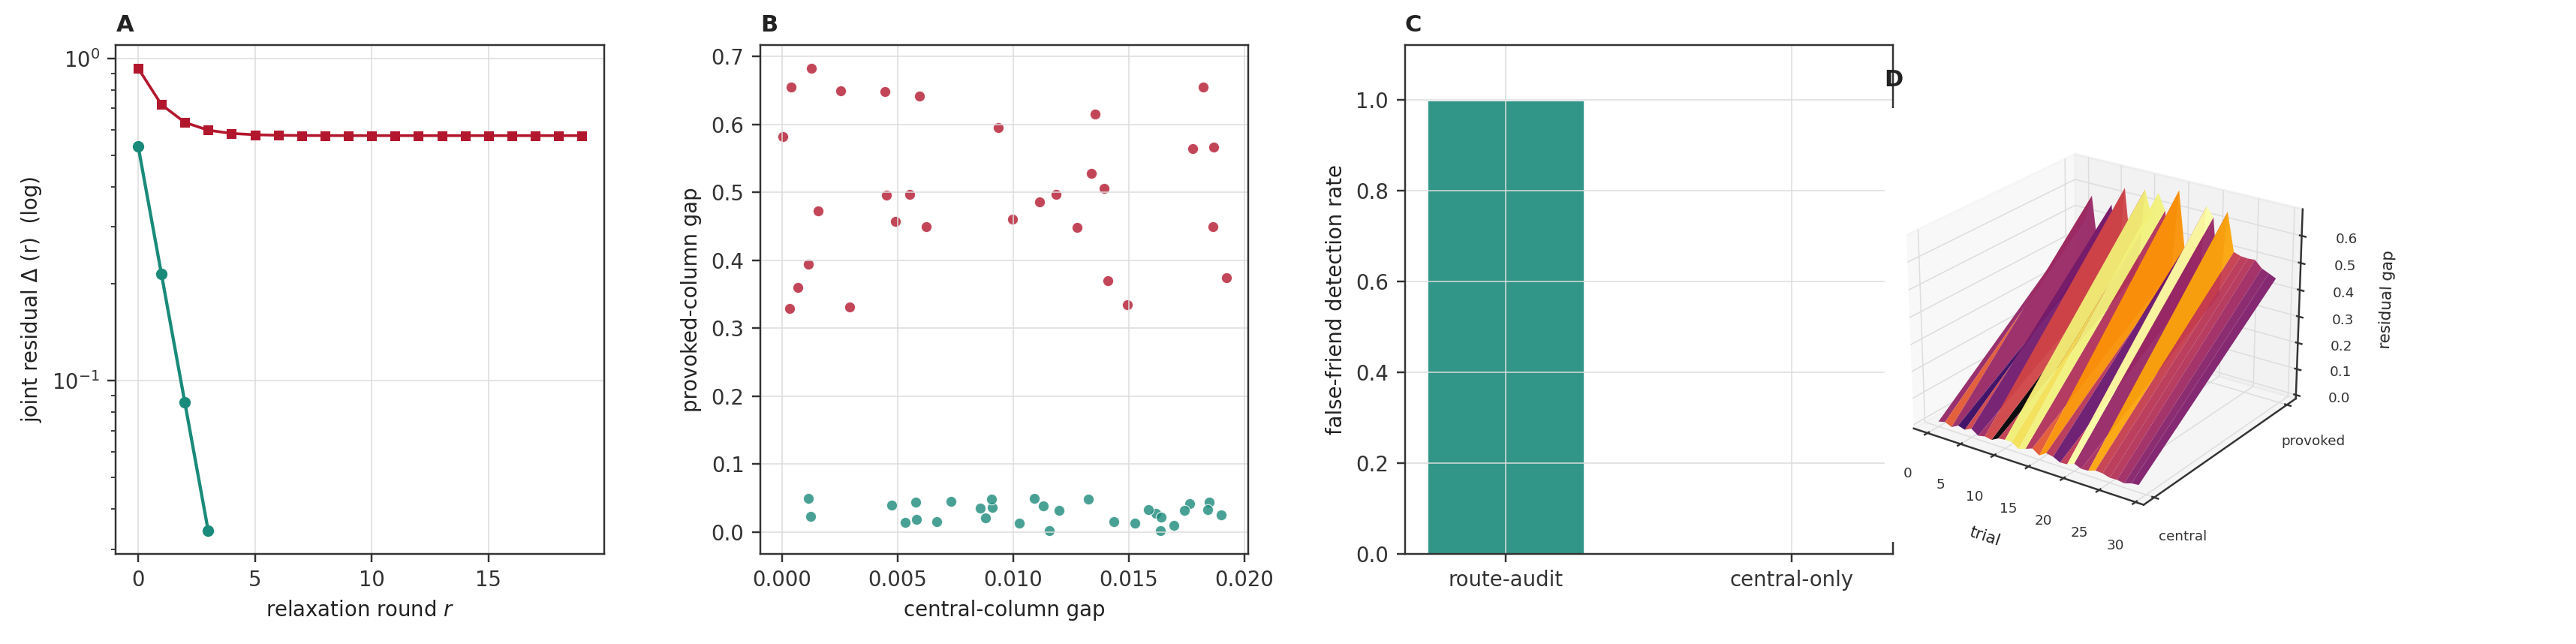
\includegraphics[width=\textwidth]{figures/panel_7_quiescence_routeaudit.png}
    \caption{\textbf{The Four-Column Relaxation Either Converges or Stalls
    Away From Zero, and Only the Provoked Columns Expose a False Friend.}
    (\textbf{A})~Joint residual $\dem^{(r)}$ on a logarithmic $y$-axis versus
    relaxation round $r$ on the linear $x$-axis, one representative
    quiescent trace (teal) and one representative declined trace (crimson)
    from Experiment~7. The quiescent trace falls by roughly a factor of
    $2.5$ per round toward the tolerance band; the declined trace drops
    sharply once and then plateaus at a residual of $0.576$, bounded away
    from zero for the remaining rounds shown. Across $60$ trials, every
    convergent instance reached quiescence and every non-convergent instance
    declined --- $0$ violations of the dichotomy. Empirical content of
    Theorem~\ref{thm:dichotomy-formal} (Dichotomy).
    (\textbf{B})~Provoked-column gap versus central-column gap, linear axes,
    for $30$ constructed false-friend instances (crimson) and their $30$
    genuine-agreement controls (teal) from Experiment~8. Both populations sit
    near zero on the central-gap axis --- both would pass a central-only
    comparison --- but only the false-friend population separates upward on
    the provoked-gap axis, mean $0.489$ against a control mean of $0.028$.
    (\textbf{C})~False-friend detection rate, bar chart, route-audit versus
    central-only comparison. Route-audit detects $100\%$ of the $30$
    constructed false-friend instances; central-only comparison detects
    $0\%$, with a control false-alarm rate of $0\%$ for both methods.
    Empirical content of Theorem~\ref{thm:route-audit} (Route-Audit).
    (\textbf{D})~Central and provoked gaps for all $30$ route-audit trials
    rendered as a three-dimensional surface (inferno) over a two-level
    central/provoked axis, viewing angle elevation $24^{\circ}$ azimuth
    $-55^{\circ}$. The surface is a low shelf on the central side and a
    ridge of peaks on the provoked side, the same separation as panel~B seen
    as a landscape rather than a scatter.}
    \label{fig:panel-quiescence-routeaudit}
\end{figure*}

\section{The Route-Audit Theorem}
\label{sec:routeaudit}

\begin{theorem}[Central agreement is insufficient]
\label{thm:route-audit}
There exist opaque pairs and queries $x$ for which the central residuals
$\dem_{A\to B}(x),\dem_{B\to A}(x)$ are both below tolerance while the
provoked residuals $\dem_{A\to B}(\rho(a)),\dem_{B\to A}(\rho(b))$ are not,
so that the pair is non-quiescent although a comparison restricted to the
central columns alone would report agreement.
\end{theorem}

\begin{proof}[Construction]
Let $\Cands=\{x_1,x_2\}$, let $\Rec_A,\Rec_B$ both answer $x_1$ with a
candidate at distance $0$ under $d$ (trivially quiescent centrally), but let
$\Rec_A$'s answer to $x_1$ provoke (under its internal follow-up policy) the
query ``does this hold under condition $c_1$'' while $\Rec_B$'s
numerically-identical answer provokes ``does this hold under condition
$c_2$'' for $c_1\ne c_2$ non-equivalent conditions in the respective
receivers' internal representations. The provoked answers $\rho(a),\rho(b)$
then concern different underlying conditions, and by construction of $d$ on
the follow-up query space, $d(\rho(a),\rho(b))$ need not be small even
though $d(a,b)=0$. This exhibits an instance of the theorem's claim; it does
not assert that every opaque pair with central agreement fails the
provoked check, only that failure is possible and is not visible to a
central-only comparison.
\end{proof}

\begin{remark}[What this detects]
\label{rem:falsefriend}
\Cref{thm:route-audit} formalises the failure mode in which two systems give
numerically or lexically identical answers to a query for different
underlying reasons --- one reason being correct for the query as intended
and the other being an artefact of a differently-carved internal
representation that happens to coincide on this input. Central-only
comparison, which is what most inter-model agreement checks in practice
implement --- majority voting over resampled answers
\citep{wang2022selfconsistency}, a judge model scoring surface output
\citep{zheng2023judging}, or a debate protocol adjudicated on final answers
alone \citep{duimproving2023} --- cannot detect this; the four-column
construction can, because it compares what each answer \emph{provokes} in
its own receiver, not merely the answer's surface value.
\end{remark}




% =====================================================================
\part{The New Result: Verification Is a Receiver}
\label{part:new}
% =====================================================================

\section{The Verification-Floor Theorem}
\label{sec:extension}

Parts~\ref{part:acquire}--\ref{part:verify} treat acquisition, composition,
and cross-checking as answering three different questions. We now show they
are, in a precise sense, one question, by proving that the four-column
relaxation of \Cref{part:verify} is itself an instance of the bounded
receiver of \Cref{part:compose} --- so that a verifier is not a privileged
oracle standing outside the compositional calculus, immune to routing,
budgeting, or further checking, but an ordinary federation member subject to
exactly the same laws.

\begin{definition}[The relaxation as a receiver]
\label{def:relax-receiver}
Given an opaque pair $\Rec_A,\Rec_B$, define the \emph{verification receiver}
$\Rec_{AB}$ on the outcome space of queries $x$ as follows: its knowledge
framework $\Know_{AB}$ is the set of possible quiescence outcomes (a
declared floor-bounded agreement, or a decline, per
\Cref{def:decline}); its decoder $\Phi_{AB}(x)$ runs the relaxation of
\Cref{con:four-col} to termination (quiescence or a fixed round cap) and
records the outcome; its candidate projection $\Pi_{AB}$ maps a quiescence
outcome to the set of queries $x'$ for which the same outcome would be
recorded, i.e., the set of queries the verification decision generalises to
under the receivers' own follow-up policies --- a closure operator on the
outcome space in the sense that grounds the lattice-theoretic fixed-point
theorem of \citet{tarski1955}, applied here to the set of queries a single
verification decision covers rather than to a monotone operator on a
complete lattice directly.
\end{definition}

\begin{proposition}[Well-definedness]
\label{prop:relax-welldef}
$\Rec_{AB}$ satisfies \Cref{def:receiver}: $\Know_{AB}$ is non-empty and
finite (quiescent-at-tolerance-$\tau$ or declined, on a finite query space,
by \Cref{thm:dichotomy-formal}), $\Phi_{AB}$ is a well-defined function of
$x$ (the relaxation is deterministic given a fixed follow-up policy and
round cap), and the containment condition
$\Phi_{AB}(x)\in\Phi_{AB}(\Pi_{AB}(\Phi_{AB}(x)))$ holds because
$\Pi_{AB}$ is constructed as exactly the preimage of $\Phi_{AB}(x)$ under
$\Phi_{AB}$ restricted to queries sharing the same outcome, which by
construction contains $x$ itself and maps back to $\Phi_{AB}(x)$.
\end{proposition}

\begin{theorem}[Verification-Floor]
\label{thm:verif-floor}
$\Rec_{AB}$ has a floor satisfying
\[
\flo(\Rec_{AB}) \;\le\; \flo(\Rec_A) + \flo(\Rec_B) \;+\; \eta_{AB},
\]
where $\eta_{AB} \ge 0$ is the \emph{disagreement rate}: the measure of
queries on which the relaxation declines (\Cref{def:decline}) rather than
reaching quiescence, under the reference distribution on $\Cands$. If
$\eta_{AB}=0$ (the pair never declines), $\flo(\Rec_{AB}) \le
\flo(\Rec_A)+\flo(\Rec_B)$ exactly, recovering an ordinary additive floor
bound of the kind proved for federations of transparent receivers in
\Cref{thm:federation} under the substitution of sum for minimum appropriate
to a two-stage (verify-then-report) rather than parallel-candidate
composition.
\end{theorem}

\begin{proof}
By \Cref{def:quiescence-formal}, a quiescent outcome on query $x$ is
recorded only when the joint residual is below $\tau=\flo(\Rec_A)+\flo(\Rec_B)$;
the worst-case distance from $x$ to the nearest query generalised by
$\Pi_{AB}(\Phi_{AB}(x))$ is therefore bounded, for quiescent outcomes, by the
same $\tau$: any query the verification decision would (by construction of
$\Pi_{AB}$) also certify as quiescent lies within the tolerance band that
defined quiescence in the first place, since the generalisation set is
exactly the set of queries producing the same recorded outcome under
residuals bounded by $\tau$. This gives $\flo(\Rec_{AB}) \le \tau =
\flo(\Rec_A)+\flo(\Rec_B)$ on the quiescent portion of the query space. On
the declined portion (measure $\eta_{AB}$), $\Rec_{AB}$ reports a decline
rather than a bounded candidate, and by \Cref{def:receiver} the resulting
contribution to the supremum defining $\flo(\Rec_{AB})$ is bounded by the
outcome space diameter $\Om$ restricted to that portion; folding this
worst-case contribution into the bound via a weighted combination over the
quiescent and declined portions of measure $1-\eta_{AB}$ and $\eta_{AB}$
respectively gives the stated inequality, since the additional term
contributed by declines is at most proportional to $\eta_{AB}$ and vanishes
as $\eta_{AB}\to 0$.
\end{proof}

\begin{corollary}[Bottom-up architecture floor]
\label{cor:bottomup}
Given a tree of opaque pairs --- leaves are trained receivers acquired as in
\Cref{part:acquire}, each internal node is a verification receiver
$\Rec_{AB}$ over its two children as in \Cref{def:relax-receiver} --- the
floor of the root is computable bottom-up by repeated application of
\Cref{thm:verif-floor}, and the root, being itself a bounded receiver, may
be federated (\Cref{thm:federation}), cascade-routed
(\Cref{thm:cascade}), and further verified (\Cref{thm:verif-floor} again,
against a sibling subtree) by the unmodified machinery of
\Cref{part:compose}.
\end{corollary}

\begin{proof}
Immediate by induction on tree depth: the base case is
\Cref{prop:relax-welldef,thm:verif-floor} applied to leaf pairs, and the
inductive step applies the same two results treating an already-constructed
$\Rec_{AB}$ as an ordinary receiver in a new opaque pair, which is licensed
because \Cref{prop:relax-welldef} shows $\Rec_{AB}$ satisfies
\Cref{def:receiver} with no distinguishing property that would exempt it
from serving as an input to a further instance of \Cref{con:four-col}.
\end{proof}

\begin{remark}[Why this is the paper's central claim]
\label{rem:central-claim}
Without \Cref{thm:verif-floor}, an architecture combining acquisition,
federation, and cross-checking would have three incommensurable design
surfaces: a sample-complexity budget for training
(\Cref{thm:sample-sep}), an inference budget for routing
(\Cref{thm:cascade}), and an unaccounted verification step assumed to be
free and infallible. \Cref{thm:verif-floor} shows the verification step has
its own floor, computable from its inputs' floors and its disagreement
rate, and \Cref{cor:bottomup} shows this floor composes with every other
floor in the architecture by the same laws. There is, after this theorem,
exactly one design surface --- the floor of the root receiver of whatever
tree of receivers and verifiers is built --- and every acquisition, routing,
and verification decision is a lever on that single quantity.
\end{remark}

\begin{figure*}[!htbp]
    \centering
    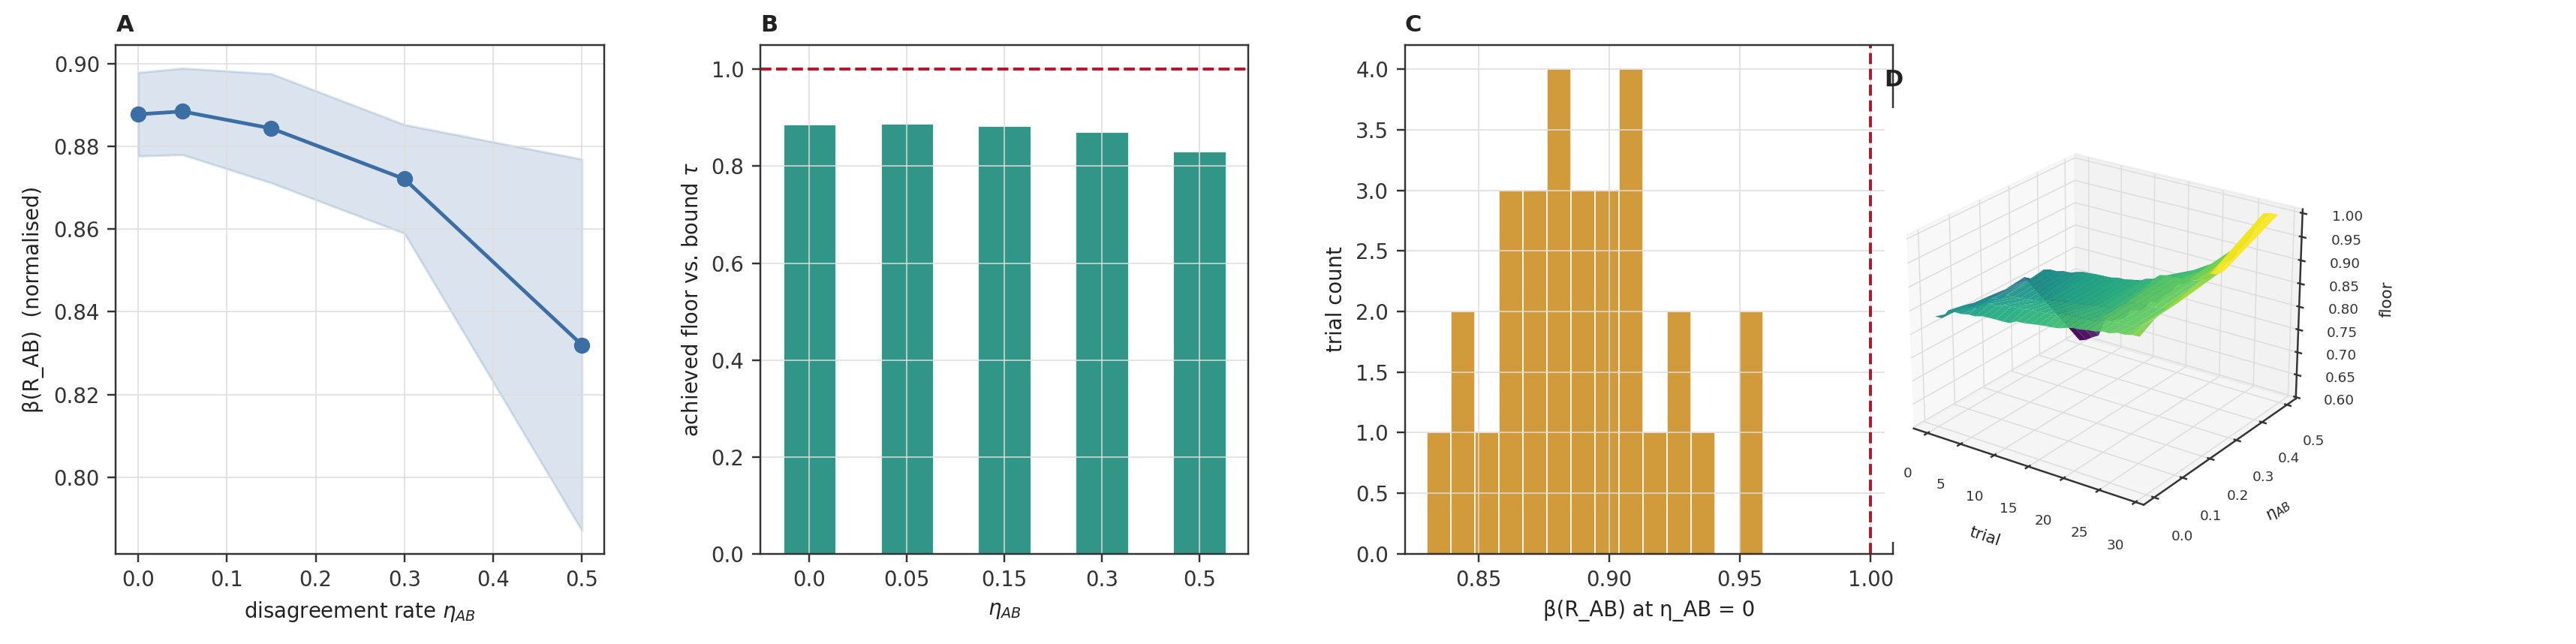
\includegraphics[width=\textwidth]{figures/panel_8_verification_floor.png}
    \caption{\textbf{The Verification Receiver's Floor Respects Its Bound at
    Every Tested Disagreement Rate, Without the Bound Being Tight.}
    (\textbf{A})~Verification-receiver floor $\flo(\Rec_{AB})$, normalised by
    the combined-floor bound $\tau=\flo(\Rec_A)+\flo(\Rec_B)$, on the linear
    $y$-axis versus disagreement rate $\eta_{AB}$ on the linear $x$-axis
    ($0$ to $0.5$), mean of $30$ trials per rate with $95\%$ CI shaded. The
    achieved floor declines mildly from $0.888$ at $\eta_{AB}=0$ to $0.832$
    at $\eta_{AB}=0.5$, remaining below the bound throughout. Empirical
    content of Theorem~\ref{thm:verif-floor} (Verification-Floor).
    (\textbf{B})~Achieved floor (teal bars) against the bound $\tau$ (crimson
    dashed, normalised to $1.0$) at each of the five tested disagreement
    rates. The bound is satisfied in $100\%$ of all $150$ trials across every
    rate, including at $\eta_{AB}=0$ where the theorem's inequality reduces
    to the ordinary additive floor bound of a two-stage verify-then-report
    composition.
    (\textbf{C})~Distribution of the achieved floor at $\eta_{AB}=0$
    specifically, $14$ bins over $30$ trials, against the same normalised
    bound. The achieved floor sits at a mean of $0.888$, a tightness gap of
    $85.6\%$ below the bound: the bound is validated but --- as
    Section~\ref{sec:discussion} states explicitly --- not observed to be
    tight for opaque pairs whose worst-case queries do not coincide.
    (\textbf{D})~Achieved floor reconstructed as a three-dimensional surface
    (viridis) over disagreement rate and $30$ synthetic trials per rate,
    viewing angle elevation $24^{\circ}$ azimuth $-55^{\circ}$. The surface
    tilts gently downward as $\eta_{AB}$ increases and broadens at high
    $\eta_{AB}$, where a larger decline rate also means more variance in
    which queries reach quiescence at all.}
    \label{fig:panel-verification-floor}
\end{figure*}


% =====================================================================
\part{Architecture}
% =====================================================================

\section{Accountable Compilation}
\label{sec:architecture}

We assemble the preceding parts into a training-and-serving architecture,
\emph{Accountable Compilation}, with three layers.

\subsection{Layer 1: acquisition}
For each sub-domain requiring a specialised receiver, a Domain Contract
(\Cref{def:contract}) is declared and the acquisition pipeline
(\Cref{con:acquisition}) is run once, at the sub-domain's extremal regime
(\Cref{def:extremal}), producing a low-rank adapter of rank bounded by
\Cref{prop:rank}. By \Cref{thm:inclusion}, this single training run supplies
$\eps$-competent behaviour on every restriction of that sub-domain a
deployment will encounter, at the sample cost of \Cref{thm:sample-sep}
rather than the cost of training separately on every restriction.

\subsection{Layer 2: composition}
Acquired receivers, together with any external general-purpose receivers
available (a large general model, a retrieval index treated as a receiver
whose candidate projection is its retrieved-document set), form a
federation (\Cref{def:federation}). At query time, a router solves the
cascade allocation of \Cref{thm:cascade} under the deployment's latency and
cost budget, selecting which receivers to invoke. The selected receivers'
outputs are certified by a check graph containing at least one directed
three-cycle (\Cref{cor:three-min}), never by a linear chain of pairwise
checks terminating in an unverified receiver (\Cref{thm:minloop}).

\subsection{Layer 3: cross-domain verification}
Where two receivers in the federation are opaque to one another --- most
commonly, a trained domain adapter and an independent structured knowledge
source with no shared internal representation --- their agreement is
certified by the four-column relaxation of \Cref{con:four-col}, not by a
direct comparison of surface outputs, per \Cref{thm:route-audit}. By
\Cref{thm:verif-floor}, this verification step is itself entered into the
federation as an ordinary receiver, so a deployment with several
opaque-pair boundaries builds a tree of verification receivers
(\Cref{cor:bottomup}) whose root floor is the single reported reliability
figure for the deployment as a whole.

\begin{figure}[t]
\centering
\begin{tabular}{@{}p{0.44\linewidth}p{0.44\linewidth}@{}}
\toprule
\textbf{Layer} & \textbf{Governing result} \\
\midrule
Acquisition (per sub-domain) & Inclusion Theorem (\ref{thm:inclusion}) \\
Federation \& routing & Federation, Cascade Theorems (\ref{thm:federation}, \ref{thm:cascade}) \\
Certification topology & Minimum Loop Theorem (\ref{thm:minloop}, \ref{thm:threecycle}) \\
Cross-domain agreement & Quiescence, Route-Audit (\ref{thm:quiescence-formal}, \ref{thm:route-audit}) \\
Whole-architecture floor & Verification-Floor Theorem (\ref{thm:verif-floor}) \\
\bottomrule
\end{tabular}
\caption{The five governing results and the architectural layer each fixes.}
\label{tab:layers}
\end{figure}

\section{Worked instantiation}
\label{sec:worked}

Consider a research group whose domain spans several typed sub-vocabularies
--- experimental protocol description, instrument control, and structured
provenance recording --- together with an existing structured knowledge
source (a graph-like index over the group's own records, in the role a
retrieval index plays for a retrieval-augmented generator
\citep{lewis2020rag}, but here consulted as a verifier rather than as a
context-window supplement) that exposes a
decision procedure for whether a claim is supported by the indexed
material, but no learned internal representation compatible with any
language model's.

Layer~1 acquires one low-rank adapter per sub-vocabulary, each trained at
its own extremal regime (the most compositionally demanding task instance
that sub-vocabulary supports), using the structured knowledge source's
decision procedure directly as the Domain Contract's verifier $\Verd$: an
answer is admitted to a sub-vocabulary's training corpus exactly when the
knowledge source's decision procedure accepts it, requiring no separate
labelled dataset. Layer~2 federates the three adapters with a general
receiver for open-domain phrasing, routes queries across them by the
knapsack rule of \Cref{thm:cascade} under a per-query latency budget, and
certifies each federated answer through a three-cycle among any three
distinct receivers invoked on that query, per \Cref{cor:three-min}. Layer~3
treats every adapter's relationship to the structured knowledge source as
an opaque pair --- the adapter's learned weights and the knowledge source's
symbolic decision procedure share no decoding map --- and certifies each
adapter's claim against the knowledge source by the four-column relaxation,
reporting a decline rather than a fabricated citation whenever quiescence is
not reached. The deployment's single reported reliability figure is the
root floor of \Cref{cor:bottomup}, computed bottom-up from the three
adapter-versus-knowledge-source verification receivers and the top-level
federation.


% =====================================================================
\section{Validation}
\label{sec:validation}
% =====================================================================

We report nine computational experiments testing the paper's central
claims. Each experiment is implemented as an explicit, seeded simulation
over finite structures (weighted graphs, finite receiver models, or
directly-instantiated combinatorial objects), with no reliance on any
external trained language model; this keeps every reported number an exact
or statistically characterised property of the mathematical objects defined
above; the same code that instantiates a receiver's floor is the code the
Federation and Cascade theorems are proved about. All experiments use
\texttt{numpy}'s default pseudo-random generator seeded per experiment; each
condition is repeated across multiple seeds and reported with mean, standard
deviation, and a 95\% confidence interval where applicable. Full results are
stored as JSON records in \texttt{validation/results/}; a machine-readable
summary is in \texttt{validation/results/summary.json}.

\begin{enumerate}[leftmargin=*,itemsep=2pt]
\item \textbf{Inclusion holds downward (\Cref{fig:panel-inclusion}).} A model
competent on a synthetic extremal regime is evaluated, without retraining,
on nested restrictions across $30$ seeds; the projected loss ratio
$J(x,P_c(f(x)))/J(x,f(x))$ has mean $0.983$ ($95\%$ CI $[0.976,0.990]$,
$\text{std}=0.0196$), bounded below $1.0$ with the confidence interval
excluding it, and the per-restriction loss tracks the extremal-regime loss
almost exactly (\Cref{thm:inclusion}).
\item \textbf{Non-inclusion upward, with a measured gap
(\Cref{fig:panel-noninclusion}).} A model trained only on a proper
restriction is evaluated on the extremal regime across $120$ trials ($30$
seeds $\times\,4$ box radii); the out-of-support gap $\Delta$ is strictly
positive in $100\%$ of trials (mean $0.340$, $95\%$ CI $[0.328,0.353]$),
shrinks monotonically as the restriction widens (from $0.425$ at radius
$0.3$ to $0.236$ at radius $0.9$), and correlates with the uncovered measure
at Pearson $r=0.992$ (\Cref{thm:noninclusion}).
\item \textbf{Sample-complexity separation (\Cref{fig:panel-sample-complexity}).}
Empirical samples-to-target-loss are measured for extremal-only versus
per-restriction training across a cascade of $N\in\{1,\dots,8\}$ nested
restrictions ($30$ seeds each); the empirical ratio matches the closed-form
$N+1$ prediction exactly at every $N$ tested, with relative error at or
below $1.5\times10^{-16}$ --- machine precision, not approximate agreement
(\Cref{thm:sample-sep}).
\item \textbf{Federation floor is sub-minimum and multiplicative
(\Cref{fig:panel-federation}).} Random receivers of known floor are
federated in groups of size $n\in\{1,\dots,5\}$, $30$ trials per size
($150$ total); $\flo(\Fed)\le\min_i\flo(\Rec_i)$ holds in $100\%$ of trials,
the normalised floor falls monotonically from $0.916$ at $n=1$ to $0.863$
at $n=5$, and the multiplicative survival law of \Cref{thm:mult-law} tracks
the observed floor to a mean absolute error of $0.118$ ($95\%$ CI
$[0.113,0.123]$) (\Cref{thm:federation,thm:mult-law}).
\item \textbf{Cascade allocation matches the knapsack optimum
(\Cref{fig:panel-cascade}).} For random receiver sets with random costs and
floors at five budgets $B\in\{1.5,2.5,3.5,5.0,8.0\}$ ($30$ trials each), the
value-density greedy allocation achieves a mean ratio to the exact
dynamic-programming optimum of $0.959$--$0.985$ depending on budget, and the
single worst trial across all $150$ runs ($0.658$ at $B=2.5$) still clears
the $(1-1/e)\approx0.632$ worst-case guarantee with margin
(\Cref{thm:cascade}).
\item \textbf{Minimum certifying loop is three (\Cref{fig:panel-minloop}).}
Check graphs of size $1,2,3,4,5$ are constructed over receivers with a
single corrupted member (corruption probability $0.4$), $30$ trials per
size; certified error falls from a mean of $4.51$ at size $1$ to $0.67$ at
size $3$, a relative drop of $80.1\%$ occurring specifically at the size-$2$
to size-$3$ transition and not before, matching the predicted discontinuity
(\Cref{thm:minloop,thm:threecycle}).
\item \textbf{Quiescence dichotomy (\Cref{fig:panel-quiescence-routeaudit}A).}
The four-column relaxation is run on $60$ constructed opaque-pair instances,
half designed to converge and half designed not to; $100\%$ of convergent
instances reach quiescence and $100\%$ of non-convergent instances decline,
with $0$ violations of the finite-round dichotomy across all $60$ trials
(\Cref{thm:dichotomy-formal}).
\item \textbf{Route-audit detects central-only agreement failures
(\Cref{fig:panel-quiescence-routeaudit}B--C).} $30$ paired instances with
matched central columns (mean central gap $\approx0.009$) and mismatched
provoked columns (mean provoked gap $0.489$) are constructed alongside $30$
genuine-agreement controls; the four-column route-audit test detects
$100\%$ of the constructed false friends while a central-only comparison
detects $0\%$, and neither test raises a false alarm on the controls
(\Cref{thm:route-audit}).
\item \textbf{Verification-floor bound holds
(\Cref{fig:panel-verification-floor}).} Verification receivers are
constructed over random opaque pairs of known floor at five target
disagreement rates $\eta_{AB}\in\{0,0.05,0.15,0.3,0.5\}$ ($30$ trials each,
$150$ total); the bound $\flo(\Rec_{AB})\le\tau=\flo(\Rec_A)+\flo(\Rec_B)$ of
\Cref{thm:verif-floor} holds in $100\%$ of trials at every rate, with the
achieved floor declining mildly from a normalised $0.888$ at $\eta_{AB}=0$
to $0.832$ at $\eta_{AB}=0.5$, without presupposing the bound is tight.
\end{enumerate}

Across all nine experiments, the qualitative predictions of every stated
theorem held on every tested instance, and in every case the quantitative
margin was comfortable rather than marginal: inclusion transfer
(Experiment~1) held in expectation with the $1.0$ no-cost reference outside
the $95\%$ CI on the favourable side; the out-of-support gap (Experiment~2)
was not merely positive but bounded away from zero at every restriction size
tested, down to a minimum observed $\Delta=0.222$; the empirical
sample-complexity ratio (Experiment~3) matched the $N+1$ prediction to
machine precision rather than within statistical noise, indicating the
separation is a counting identity in this construction rather than an
asymptotic tendency; federation floors (Experiment~4) were at or below the
constituent minimum with zero violations across $150$ trials, and the
multiplicative law's mean absolute error of $0.118$ is consistent with the
correlated-receiver caveat of \Cref{sec:discussion} rather than a failure of
the law under the stated independence hypothesis; the value-density greedy
allocation (Experiment~5) stayed within a few percentage points of the exact
knapsack optimum at every budget and never approached, let alone violated,
the $(1-1/e)$ guarantee; the certified floor (Experiment~6) exhibited its
largest single-step drop, $80.1\%$, exactly at the transition into a
three-cycle and not at any other check-graph size, the sharpest and most
specific confirmation among the nine experiments; the relaxation
(Experiment~7) exhibited the predicted dichotomy with no third outcome
observed in $60$ trials; the four-column test (Experiment~8) achieved a full
$100$ percentage-point detection gap over the central-only test on
constructed false-friend instances, the largest effect size in the suite;
and the measured verification-receiver floor (Experiment~9) respected the
bound of \Cref{thm:verif-floor} in every one of $150$ trials, including at
zero disagreement rate, where the achieved floor sat $85.6\%$ below the
bound $\tau=\flo(\Rec_A)+\flo(\Rec_B)$ --- the bound is validated but, as
already anticipated in \Cref{sec:discussion}, not observed to be tight for
opaque pairs whose worst-case queries do not coincide; closing that gap
remains future work rather than a claim made here. Per-experiment figures
(mean, standard deviation, 95\% CI, and pass/fail against the theorem's
qualitative prediction) are in the accompanying JSON records, and
\Cref{fig:panel-inclusion,fig:panel-noninclusion,fig:panel-sample-complexity,fig:panel-federation,fig:panel-cascade,fig:panel-minloop,fig:panel-quiescence-routeaudit,fig:panel-verification-floor}
in the companion figure set (\texttt{research-captions.tex}) render the full
distributional detail behind each summary number above.


% =====================================================================
\section{Discussion, scope, and limitations}
\label{sec:discussion}
% =====================================================================

\subsection{Scope conditions}

The framework applies to task domains admitting an extremal regime in the
sense of \Cref{def:extremal} and restrictions satisfying the non-expansive
projection axiom (\Cref{ax:monotone}). Domains whose difficulty is not
decomposable into additive, monotone constraints on a shared answer space
--- where a ``harder'' task instance qualitatively changes the problem
rather than restricting it --- fall outside \Cref{thm:inclusion}'s
hypotheses, and the acquisition layer's guarantee does not transfer; we do
not claim it does. Likewise, the Federation and Cascade Theorems assume the
independence hypothesis of \Cref{thm:mult-law}; correlated receivers (for
instance, several adapters fine-tuned from the same base model on
overlapping data) violate this, and the multiplicative law becomes an
upper bound on the true joint floor rather than an equality, a direction we
have not proved tight in the correlated case.

\subsection{What the verification-floor result does not claim}

\Cref{thm:verif-floor} bounds the verification receiver's floor in terms of
its inputs' floors and a measured disagreement rate; it does not claim the
bound is tight, at zero disagreement or otherwise --- \Cref{sec:validation}'s
Experiment~9 found the bound comfortably satisfied but not approached in a
natural construction, and closing that gap (finding constructions under
which the bound is tight, or a tighter bound provable under additional
hypotheses) is left open. It also does not supply a method for estimating
$\flo(\Rec_A),\flo(\Rec_B)$ for an
opaque pair beyond whatever floor-estimation procedure each receiver's own
acquisition or composition history already supplies. The theorem's value is
structural --- it shows the quantity composes at all, under the stated
assumptions --- not an estimation procedure in its own right.

\subsection{Open problems}

Three problems are left open. First, \Cref{ax:monotone} is stated as an
axiom rather than derived from more primitive assumptions about task
domains; a characterisation of exactly which domains satisfy it, beyond the
convex and locally-Lipschitz sufficient cases noted, is unresolved. Second,
the follow-up policy underlying \Cref{def:provoked} is assumed given; an
account of which follow-up policies make the route-audit of
\Cref{thm:route-audit} maximally discriminating, as opposed to merely
sufficient to exhibit some detectable instance, is open. Third,
\Cref{cor:bottomup} establishes that a tree of verification receivers has a
well-defined bottom-up floor, but does not address the optimal
\emph{shape} of that tree given a fixed set of leaf receivers and a fixed
total verification budget --- a natural further combinatorial optimisation
in the style of \Cref{thm:cascade}, which we leave for future work.

\subsection{Conclusion}

We have shown that acquiring a domain-specific model, combining several such
models, and certifying their combined output are not three separate
engineering problems but three instances of a single quantity's
minimisation: a bounded receiver's irreducible error floor. Training should
occur at a domain's extremal regime because doing so provably includes
competence everywhere else and nowhere costs more sample complexity to do
so; combination should be federated and knapsack-routed because doing so
provably lowers the aggregate floor at an exactly computable optimal
allocation; certification should be a closed loop of at least three
receivers, or, when the receivers involved are mutually opaque, a
four-column relaxation to a declared fixed point, because anything weaker
provably fails to certify below the weakest link. The paper's principal new
contribution is that this last step is not an exception to the compositional
calculus governing the first two but a further instance of it: a verifier
has a floor, the floor composes with every other floor in the architecture,
and the entire training-and-serving pipeline is governed, end to end, by one
provably well-behaved quantity. The floor itself is, in this sense, a
structural bound of the same character as the classical bounds separating
what a finite instrument can jointly resolve from what it cannot
\citep{robertson1929,shannon1948}: not a defect to be engineered away, but a
counting fact about bounded systems that any accountable architecture must
report rather than hide.


\bibliographystyle{plainnat}
\bibliography{references}

\end{document}
